\documentclass[a4paper,11pt]{article}
\pdfoutput=1 % if your are submitting a pdflatex (i.e. if you have
             % images in pdf, png or jpg format)

\usepackage{jinstpub} % for details on the use of the package, please
                     % see the JINST-author-manual

\usepackage[utf8]{inputenc}

\usepackage{lineno}
\usepackage{color}
\newcommand{\todo}[1]{\textcolor{red}{{#1}}}

\linenumbers

\title{\boldmath Commissioning and performance in beam tests of the highly granular SiW-ECAL technological prototype for the ILC}

% e-mail addresses: only for the forresponding author
\emailAdd{irles@lal.in2p3.fr}
%\collaboration[]{on behalf of the CALICE collaboration}


\abstract{
  High precision physics at future colliders as the International Linear Collider (ILC) require unprecedented high precision in the determination
  of the energy of final state particles.
  The needed precision will be achieved thanks to the Particle Flow algorithms (PF) which require highly granular and hermetic calorimeters systems.
  The Silicon-Tungsten Electromagnetic Calorimeter (SiW-ECAL) technological prototype
  design and R\&D is tailored to the baseline design of the ECAL of the International Large Detector (ILD) for the ILC.
  In this document we present the latest news on R\&D of such prototype with fully embedded very front-end (VFE) electronics.
  Special emphasis is given to the presentation and discussion of the commissioning of the prototype
  for beam test and to the performance of the device in such beam test carried at DESY in June 2017.
}


\keywords{Calorimeter methods, calorimeters, Si and pad detectors}


\begin{document}
\maketitle
\flushbottom


\section{Introduction}

Future accelerator based particle physics experiments
require very precise and detailed reconstruction of the final states produced
in the beam collisions. A particular example is the next generation of $e^{+}e^{-}$
linear colliders such the ILC\cite{Behnke:2013xla,Baer:2013cma,Adolphsen:2013jya,Adolphsen:2013kya,Behnke:2013lya}.
This project will provide collisions of polarized beams with centre-of-mass energies ($c.m.e$) of 250 GeV - 1 TeV.
These collisions will be studied by two multipurpose detectors:
the International Large Detector (ILD) and the Silicon Detector (SiD)\cite{Behnke:2013lya}.
Another example of an $e^{+}e^{-}$ collider project is the Compact Linear Collider (CLIC)
project\cite{Aicheler:2012bya,Linssen:2012hp,Lebrun:2012hj}
which will produce collisions with $c.m.e$ of 380 GeV - 3 TeV
with a detector featuring similar design than the ILD and SiD.
Both projects will explore with unprecedented precision the origin of the electroweak symmetry breaking and new physics beyond the standard model by exploring final states with heavy bosons (W, Z  and H) and fermions ({\it i.e.} heavy quarks as $c$, $b$ and $t$).

To meet the required precision levels, these detectors will be based on the Particle Flow (PF) techniques\cite{Brient:2002gh,Morgunov:2004ed,Sefkow:2015hna}.
These techniques rely on single particle separation to make possible the choice of the best information available
in the full detector to measure the energy of the final state objects: {\it i.e.} the charged particles momentum is better measured by the tracking system
the photons energy by the electromagnetic calorimeter and the neutral hadrons energy by the full calorimeter system.
In that way the poor resolution of the calorimeter systems (compared with trackers) will  only have a reduced impact in the overall reconstruction.
For this purpose, detectors optimized for PF algorithms have some requirements, summarized here:

\begin{itemize}
\item a highly efficient and "transparent" tracking system between the interaction point and the calorimetry systems;
\item highly granular ({\it imaging calorimetry}) and compact calorimeter systems featuring minimum dead material;
\item and high power of particle separation\footnote{
For that reason the calorimeter systems at ILD will be placed inside the magnetic coil
providing magnetic fields of 3.5 T}.
\end{itemize}

The R\&D of highly granular calorimeters for future linear colliders is conducted within the CALICE collaboration and, for now on, we refer the reader to \cite{Sefkow:2015hna} for further information about PF and the CALICE R\&D.

In this document we will focus in the description of the silicon-tungsten electromagnetic calorimeter,
SiW-ECAL, its commissioning and its performance in beam test.
The SiW-ECAL is the baseline choice for the ILD ECAL. It consists in a detector (in the barrel region) of 24 $X_{0}$ of thickness which corresponds to $\sim 1~\lambda_{I}$ (interaction length).
It has silicon (Si) as active material and tungsten (W) as absorber material.
The combination of Si and W choices  makes possible the design and construction
of a very compact calorimeter with highly granular and compact active layers.
It will consist of an alveolar structure of carbon fiber into which modules called SLABs made of tungsten
plates and the active sensors will be inserted. The very-front-end (VFE) electronics will be
embedded in the SLABs. The silicon sensors will be segmented
in squared cells (or channels) of 5x5 mm: a total of $\sim 100$ million channels will constitute the ECAL for ILD.
The desired signal dynamic range in each channel goes from 0.5 MIP to 3000 MIPs.
To reduce overall power consumption, the SiW-ECAL will exploit the special bunch structure
foreseen for the ILC: the $e^{+}e^{-}$ bunchs trains will arrive within
acquisition windows of $\sim$ 1-2 ms width separated by $\sim$ 200 ms. During the idle time, the bias currents of the electronics will be shut down.
This technique is usually denominated power pulsing. In addition to this, to cope with the large amount of channels, the calorimeters should work in self-trigger mode (each channel featuring an internal trigger decision chain) and zero suppression mode. 

The first SiW-ECAL prototype was the so called SiW-ECAL physics prototype.
It was successfully tested at DESY, FNAL and CERN running together with another prototype from the CALICE
collaboration, the analogue hadronic calorimeter AHCAL, delivering the proof of concept of PF calorimetry.
For the physics prototype, the VFE was placed outside the active area with no particular constraints in power consumption.
It consisted of 30 layers of Si as active material alternated with tungsten plates as absorber material.
The active layers were made of a matrix of 3x3 Si wafers. Each of these wafers was segmented in matrices of
6x6 squared pixels of 1x1 $cm^{2}$.
The prototype was divided in 3 modules of 10 layers with different W depth per layer in each of these modules
(0.4, 1.6 and 2.4 $X_{0}$) making a total of 24 $X_{0}$.
Published results proving the good performance of the technology and the PF can be found in references~\cite{Adloff:2011ha,Anduze:2008hq,Adloff:2008aa,Adloff:2010xj,CALICE:2011aa,Bilki:2014uep}.

\section{The SiW-ECAL engineering prototype}


The new generation prototype is called the SiW-ECAL technological prototype and it addresses the main technological challenges: compactness,
power consumption reduction through power pulsing and VFE inside the detector close to real ILD conditions.
It will also provide data to deeply study the PF and provide input to tune the Monte Carlo programs.

\subsection{Silicon sensors}
\label{sec:wafers}

The sensors consist on float zone silicon wafers 320$\mu$m thick with high resistivity (larger than 5000 $\Omega\cdot$cm). The size of the wafer is $9\times9$ cm$^{2}$ featuring an array of 256 PIN diodes of $5\times5$ mm$^{2}$. A MIP traversing the PIN parallel to its normal will create $\sim$ 80 $h^{+}e^{-}$ pairs per $\mu$m which corresponds to 4.1 fC if the particle traverses the 320$\mu$m perpendicularly to its larger surface.

The original design of the silicon wafers included an edge termination made of floating guard-rings.
It was observed in beam test\cite{Cornat:2015eoa,Cornat:2009zz} that the capacitive coupling between such floating guard-rings 
and the pixels at the edge was not negligible in tests with high energy beams (pions and electrons with energies larger than 20-40 GeV).
This coupling lead to fake events in which, at least,
the channels in the four edges of the wafer are triggered at the same time. 
This is why these events are so often called squared events. 
An R\&D program together with Hamamatsu Photonics (HPK Japan) was conducted to study the guard-rings design 
as well as the internal crosstalk. As outcome of this R\&D program, the technological prototype 
is equipped with silicon wafers with:

\begin{itemize}
\item \todo{N wafers type-X with guard-rings of XXX characteristics (continuous, segmented, segmented smaller??)}
\item \todo{N wafers type-Y without guard rings and the width of the peripheral dead areas lower than 500 $\mu$m thanks to the use of stealth dicing technique.}
\end{itemize}

For the wafers \todo{type-Y}, the amount of squared events is expected to be reduced by, at least, a \todo{factor XXX}. In both cases, 
for interaction with low energy particles as the delivered at the DESY beam test facility (see Section \ref{sec:beamtest}) the
amount of squared events is expected to be negligible, therefore we will not do any differentiation 
of our results depending on the wafer type mounted in the detector.

\todo{ Is this needed? If so, what are the right plots to show?} Before the assembly of the sensors in the detector, these are characterized one-by-one by measuring the leakage current (of the order of 1 nA per single diode) 
as a function of the bias voltage (I-V curve), the full depletion voltage (of 40 V) extracted from C-V curve and
the stability in time (leakage current versus time at a nominal bias).
%The single diodes have capacitances of 8 $pF$.

\begin{figure}[!t]
\centering
\begin{tabular}{l}
  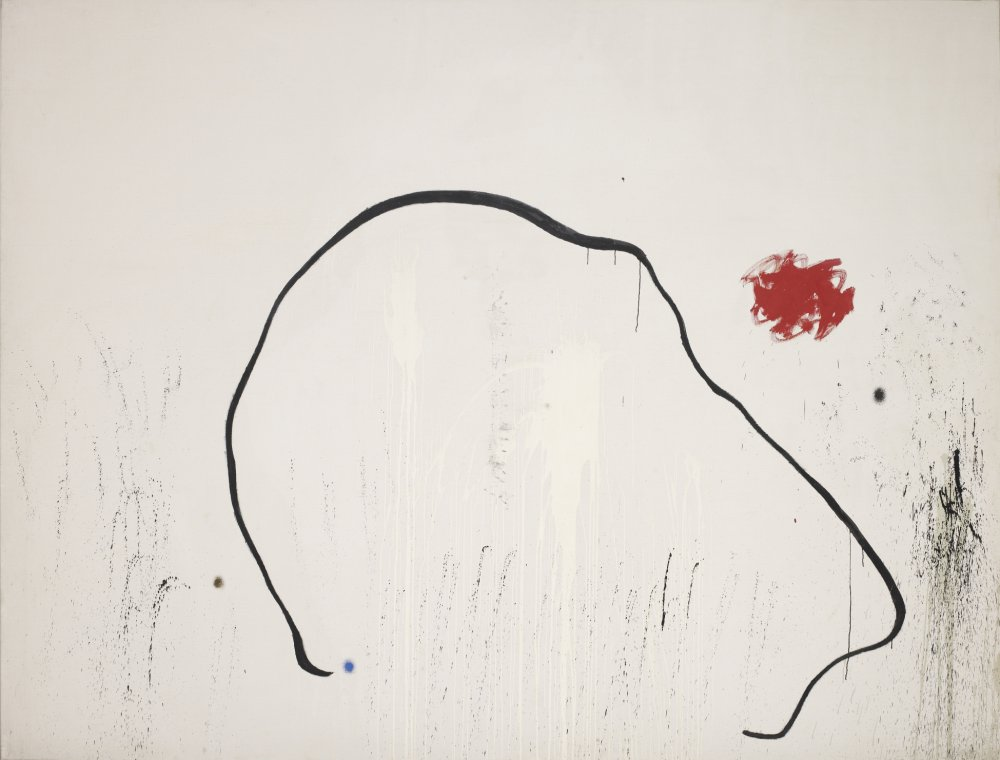
\includegraphics[width=3.0in]{figs/test.jpg} \\
  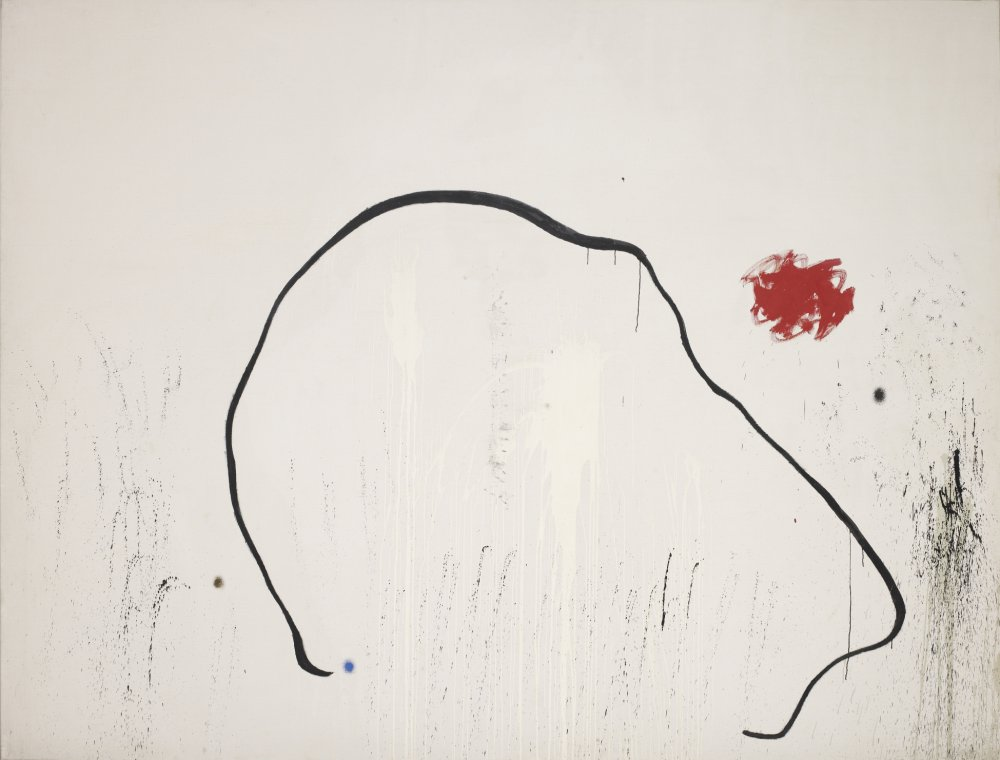
\includegraphics[width=3.0in]{figs/test.jpg} \\
  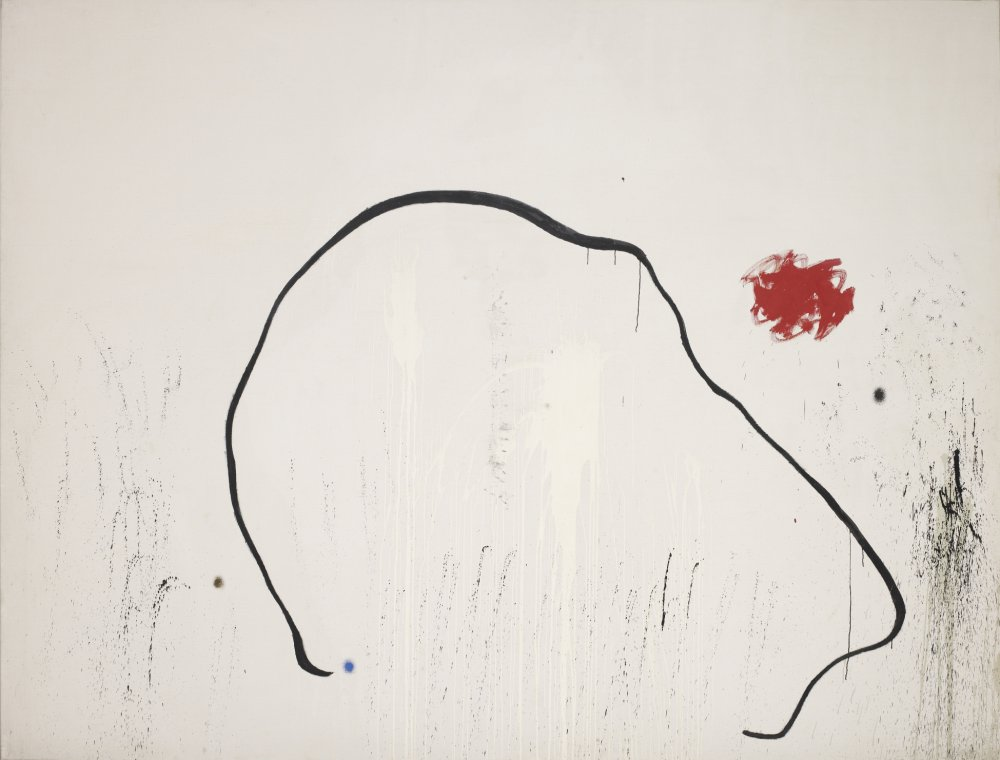
\includegraphics[width=3.0in]{figs/test.jpg}
\end{tabular}
\caption{I-V curve, C-V curve, leakage current vs time. \todo{Temporary picture: La Esperanza del Condenado, J. Miró}}
\label{shortslab}
\end{figure}

\subsection{SKIROC: Silicon pin Kalorimeter Integrated ReadOut Chip}
\label{sec:skiroc}

SKIROC\cite{Callier:2011zz} (Silicon pin Kalorimeter Integrated ReadOut Chip) is the very front end ASIC designed for the readout of the Silicon PIN didoes.
It consists of 64 channels in AMS 0.35 $\mu$m SiGe technology. Each channel comprises a low noise charge preamplifier of variable gain followed by two lines:
a fast shaper for the trigger decision and a set of dual gain slow shaper for charge measurement. 
The gain can be controlled by modifying the feedback capacitance during the configuration of the detector.
With the slowest gain, 6pF, the ASIC will handle a linear dynamic range from 0.1 to up to 1500 MIPs 
(a slightly less than the desired final value for the ILC). 
Finally, a Wilkinson type analogue to digital converter fabricates the digitized charge deposition that can be readout. 
Once one channel is triggered, the ASIC reads out all 64 channels adding a bit of information to tag them as
triggered or not triggered and the information is stored in 15 cell deep physical switched capacitor array (SCA).
The trigger threshold can be controlled both globally and locally (channel by channel) although the
dynamical range for the channel by channel option is too small in the SKIROC version 2 due to a mistake in the development. The trigger holds the voltage of the two slow shapers with a tunable delay and also
holds the voltage swept with the slow clock trigger to obtain timing information. 

The SKIROC ASICs can be power-pulsed by taking advantage of the ILC spill structure: 
the bias currents of the ASIC can be switched off during the idle time between bunch trains.
With this method, the ASIC is able to reduce its power consumption down to 25 $\mu$W per channel,
meeting the ILC requirements. All the results shown in this paper are obtained using the power pulsing feature.

Every ASU of the SiW-ECAL prototype is equipped with 16 SKIROCs version 2. A new version, 2a, has been produced and will be used to equip new layers currently in production.
In addition, a new generation of the ASIC, SKIROC3, is foreseen for the final detector construction.
In contrast with SKIROC2/2a, the new ASIC will be fully optimized for ILC operaton, {\it i.e.} full zero suppression, reduced power consumption etc.

\begin{figure}[!t]
  \centering
    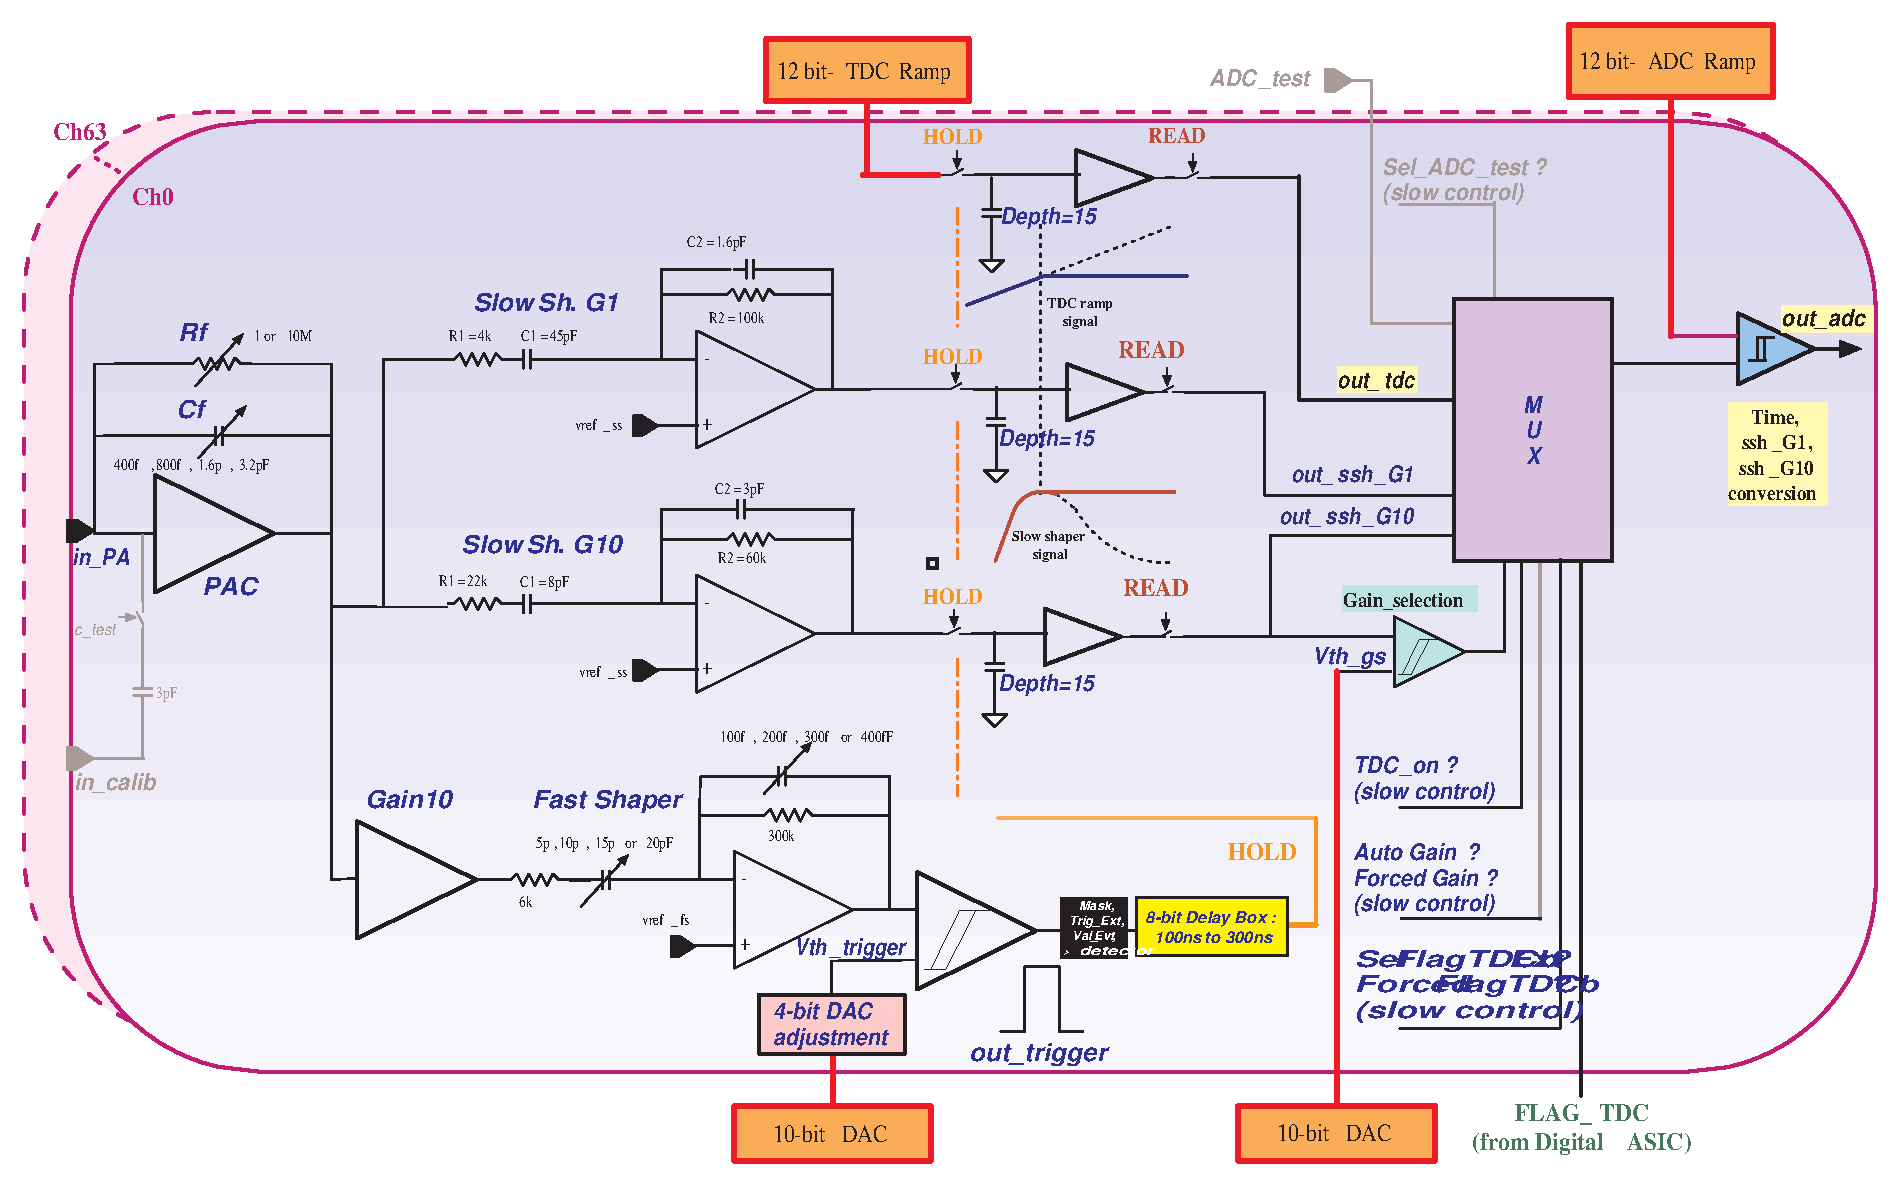
\includegraphics[width=4in]{figs/skiroc2_block.eps}
\caption{The schematics of the analog part of SKIROC2. \todo{High-stack picture (right bottom corner)}}
\label{SKIROC2}
\end{figure}

\subsection{Active Sensor Units}
\label{sec:ASU}

\begin{figure}[!t]
  \centering
  \begin{tabular}{l}
    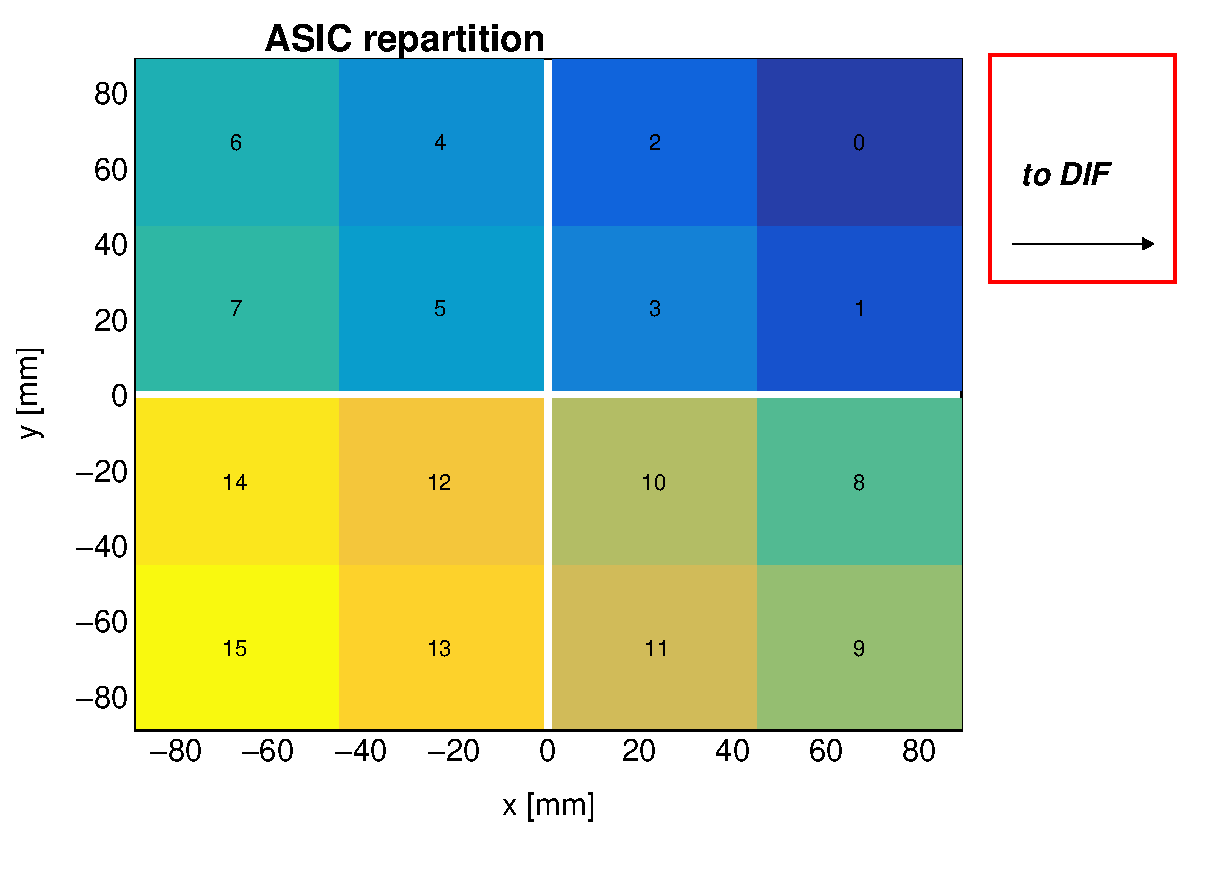
\includegraphics[width=4in]{figs/ASU_geometry1.eps}  \\
    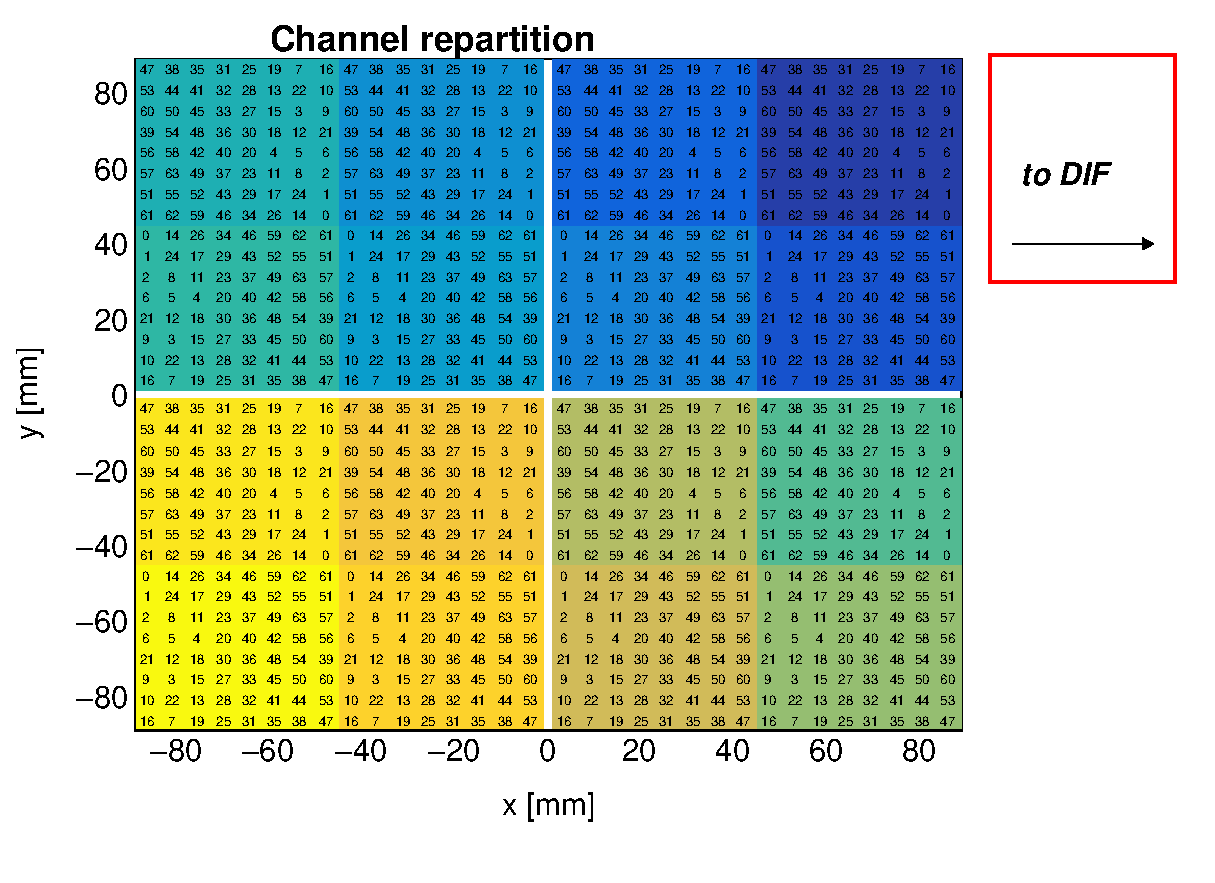
\includegraphics[width=4in]{figs/ASU_geometry2.eps}  \\
  \end{tabular}
  \caption{Repartition of the ASIC (up) and channels (down) in one ASU. In this perspective, the Si-Sensors are in glued in the back. The channels are separated (in x and y) by 5.5 mm.
    The empty cross in the middle of the ASU corresponds to the 1 mm separation between the sensors.}
\label{ASU}
\end{figure}

The entity
of sensors, thin PCB (printed circuit boards) and ASICs (application-specific integrated circuits) is called Active Signal Units or ASU.
An individual ASU has a lateral dimension of 18x18 cm$^{2}$ and has glued onto it 4 silicon wafers (currently with a thickness of 320 $\mu$m). The high voltage is delivered to the wafers using a HV-kapton sheet that covers the full extension of the wafers.
The ASUs are equipped
further with 16 ASIC for the read out and features 1024 square pads (64 per ASIC) of 5x5 mm. The channels and ASICs are distributed along the ASU as shown in Figure \ref{ASU_geometry}

The readout layers of the SiW-ECAL consist of a chain of ASUs and an adapter board
to a data acquisition system (DAQ) at the beginning of the layer.
This adapter board is called SMBv4
and it also serves as a place to sit the power connectors (low voltage to power the analog and digital
parts of the ASIC and high voltage to bias the PIN diodes) and the super capacitances used for the power pulsing. 
These capacitances of 400mF with 16 m$\Omega$ of equivalent serial resistance. 
The purpose of these capacitances is to provide local storage 
of the necessary charge to avoid the transport of current pulses over long cables, 
ensuring in this way the stability of the ASICs during the acquisition. 

Currently, the technological prototype layers are built with version of PCB called FEV11 with 16 SKIROC (see Section \ref{sec:DAQ}).
The FEV11 thickness is 1.6 alone and 2.7 mm including the ASICs in its current packaging: 1.1 mm thick LFBGA package.
Figure \ref{shortslab} (left) shows a picture of a full equipped short slab with FEV11 ASU.
There are ongoing R\&D activities in an alternative PCB design in which the ASICs
are directly placed on board of the PCB in dedicated cavities.
The ASICS will be in semiconductor packaging and wire bonded to the PCB. This is the so-called COB (chip-on-board) version of the ASU.
A small sample of FEV11\_COBs (same connexion pattern with the interface card than FEV11)
with a total thickness of 1.2 mm has been produced and tested in the laboratory
showing its readiness for tests with particle beams. A sample can be seen in Figure \ref{shortslab} (right).

\begin{figure}[!t]
  \centering
  \begin{tabular}{ll}
    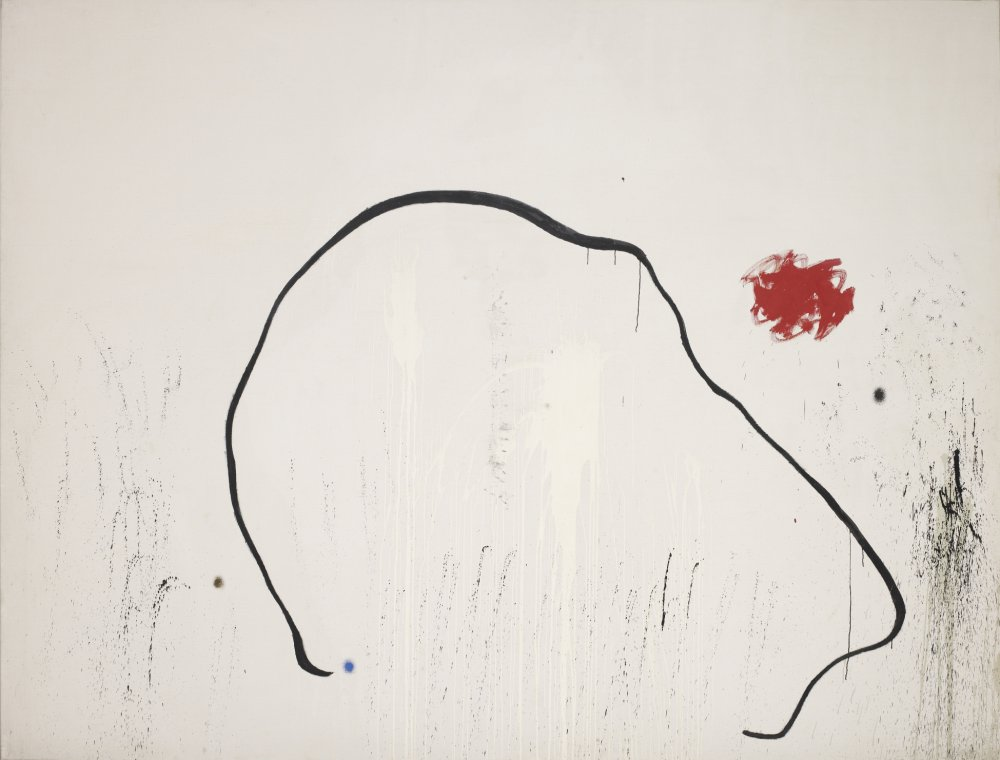
\includegraphics[width=2.8in]{figs/test.jpg} & \includegraphics[width=2.8in]{figs/fev11_cob.png} 
  \end{tabular}
  \caption{Left \todo{Temporary picture: La Esperanza del Condenado, J. Miró}: Open single SLAB with FEV11 ASU, 16 SKIROC, interface card and DIF visibles. The silicon sensors are glued to the PCB in the other side.
  Right: two FEV11\_COB boards with 16 SKIROC2a wire bonded. The ASICs are protected with watch glasses.}
\label{ASU}
\end{figure}

\subsection{Data AcQuisition system}
\label{sec:DAQ}

The design of the subsequent chain of the data acquisition (DAQ)\cite{Gastaldi:2014vaa} system is inspired by the ILC.
Current DAQ consists of three modules which are designed to be generic enough to cope with other applications.
The first module is the so called detector interface (DIF) which is placed at the beginning of each layer holding up to 15 ASUs.
All DIFs are connected by single HDMI cables to the concentrator cards: Gigabit Concentrator Card (GDCC).
The HDMI connection is used to transmit both slow control and data readout.
One GDCC controls up to 7 DIFs collecting all data from them and distributing to them the system clock and fast commands.
The most downstream module is the clock and control card (CCC).
The CCC provides a clock, control fan-out of up to 8 GDCCs and accepts and distributes external signals (i.e. spill signals).

The whole system is controlled by the Calicoes and the Pyrame DAQ software version 3~\cite{Rubio-Roy:2017ere,Magniette:2018wdz}.
The Pyrame framework provides basic blocks (called modules) of control-command or data acquisition.
Calicoes is specific the implementation of these blocks for control-command and data acquisition of the SiW-ECAL prototype. 
This new version of the DAQ software implements a new mechanism to allow any module to treat and publish data in real time. 
Those data are made available to any requesting module, in particular to a new online monitor module developed
for this beam test, allowing for quick online checks of the data quality and integrity.

\subsection{Setup}
\label{sec:setup}

The prototype tested in beam is composed of 7 layers consisting in one short SLAB each.
A short SLAB is made of: one single ASU FEV11 equipped with 16 SKIROC2 and 4 wafers glued on the other side (1024 channels);
an interface card SMBv4; and a DIF. All these elements sit on a "U" shape carbon structure to protect the wafers.
The full system is then covered by two aluminum plates to provide electromagnetic shielding and mechanical stability.
The 7 layers are supported by a PVC and aluminum structure that in which can be inserted to 10 layers.
The distance between two layer slots is 15 mm and this space is used to place tungsten plates of different thicknesses.
For the beam test described in Section \ref{sec:beamtest}, the layers were placed in positions 1-6 and 10.
During the commissioning, the slabs have been tested both inside and outside of the structure.
A photograph showing the prototype can be seen in Figure \ref{proto}. The ASICs and channels
are labeled with numbers following design and DAQ criteria: from 0-16 in the case of the ASICs and from 0-63 in the case of the channels.
%The mapping from this numbering scheme to real positions in the ASUs is shown in the right plot of Figure \ref{proto}. 

\begin{figure}[!t]
\centering
\begin{tabular}{l}
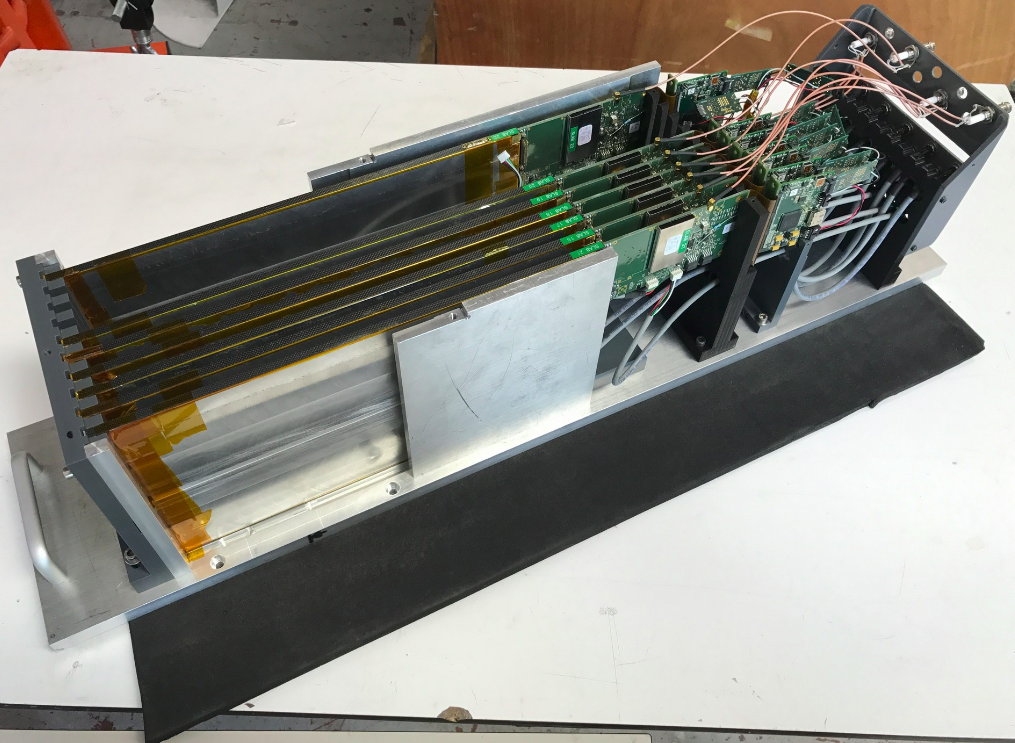
\includegraphics[width=4.0in]{figs/proto.png} 
\end{tabular}
\caption{Prototype with 7 layers inside the aluminum stack.}
\label{proto}
\end{figure}


\section{Commissioning of the detector}
\label{sec:commissioning}

This beam test was prepared by a careful and comprehensive commissioning comprising:
the debug of the
single SLABSs with special emphasis in the control of the noise and the study of the
prototype performance in cosmic rays tests.

The SKIROC2 has been already commissioned for previous experiences (see for example the 
references \cite{Amjad:2014tha,Suehara:2018mqk}). 
Therefore, all the settings used for the SKIROC2 to obtain 
the results described in this paper are motivated by previous experiences. 
For example, the value of 1.2pF for the preamplifier. 
With this gain, the SKIROC2 ensures a linearity better than 90\% 
for 0.5-200 MIPs, which is optimal for 
electromagnetic showers created by few GeV 
electrons or positrons. The delay of the trigger signal is the same than in 
reference \cite{Amjad:2014tha,Suehara:2018mqk}: 130 DAC for all ASICS. 
This value was chosen by selecting the delay in which an injected signal
of few MIPs of value get the maximum value of ADC. %Finally, the value of the
%compensation capacitance at the output of the preamplifier has been set to 6pF instead of 
%4pF to prevent overshots and ripples of the signal used as input to the trigger
%decision and ADC lines. 


\subsection{Optimization of noise levels}
\label{sec:comm_noise}

The purpose of this phase was to monitor and control the
noise levels of the prototype. The commissioning includes the definition of trigger threshold values and a list of noisy channels to be masked.
Studying and control the noise levels in an self-triggered and high-granularity calorimeter
is crucial since noisy channels may saturate the DAQ faster than physical signals.
Two different types of noise were identified:
randomly distributed (in time) noisy channels 
and noise bursts affecting to all layers at the same time.

The first type of noise source (randomly distributed in time)
forced us to define a list of channels to be masked in all 
layers. Again, two different type of noisy channels have been identified. 
The first group is compose by randomly distributed (in space) channels which 
slightly larger number of triggers than the others. The second group is made of
a fixed list of channels, all in the same positions for all SLABs, that were giving
underflowed ADC triggers at high rates. 

The channels associated to "underflowed-noise" events were identified by means of the online monitoring
tools. Some preliminary inspections of the FEV11 layout hint that
the cause of this "underflowed-noise" events may be in an improvable routing of the
lines from the PIN pad to the SKIROC. 
For this reason, if a given channel appeared to be associated 
to "underflowed-noise" events in one of the SLABs, 
it was masked in all of them, taking in this way the most conservative solution.
For example, all channels number 37 were masked in all ASICs.
More studies in this respect are to come.

The list of the noisy channels randomly distributed in time and space was
defined by means of dedicated data taking runs. 
These runs were characterized by: their short acquisition windows (of 2.5 ms, only 1.1 ms 
of effectively data taking time), their low
spill frequency (5 Hz) to minimize the chances of having real events due to cosmic rays 
hitting the detector during the
data taking; and the relatively high trigger threshold values between 250 and 400 DAC 
(which is equivalent to $\sim$0.5-2 MIP, see Section \ref{sec:comm_trigger} for more 
information). The full process was an iterative process starting with several repetitions
of runs at a high threshold value and then some iterations at lower threshold each up to 250 DAC. 
In every of there iterations, the channels identified as noisy were masked.
A full run involved 3-5 threshold values and at least two repetitions per value.
Again, we decided to follow a conservative approach for list the noisy channels to be masked:
if the channel was triggered at rates larger than 0.5-1\% of the total number of triggers it was added to the list.

In addition to the different noisy channel types described above, we also have
masked full sectors of the SLABs if an ASIC was faulty (at least 70\% of channels 
listed as noisy) or if a Si-wafer was misworking (high leakage currents). In these cases 
and in all mentioned above, the masking involved two steps: disabling of the trigger and 
the disabling of the power of the preamplifier of that channel. A summary of the results of the masking procedure is shown in Figure \ref{noisycells}.

\begin{figure}[!t]
  \centering
  \begin{tabular}{l}
  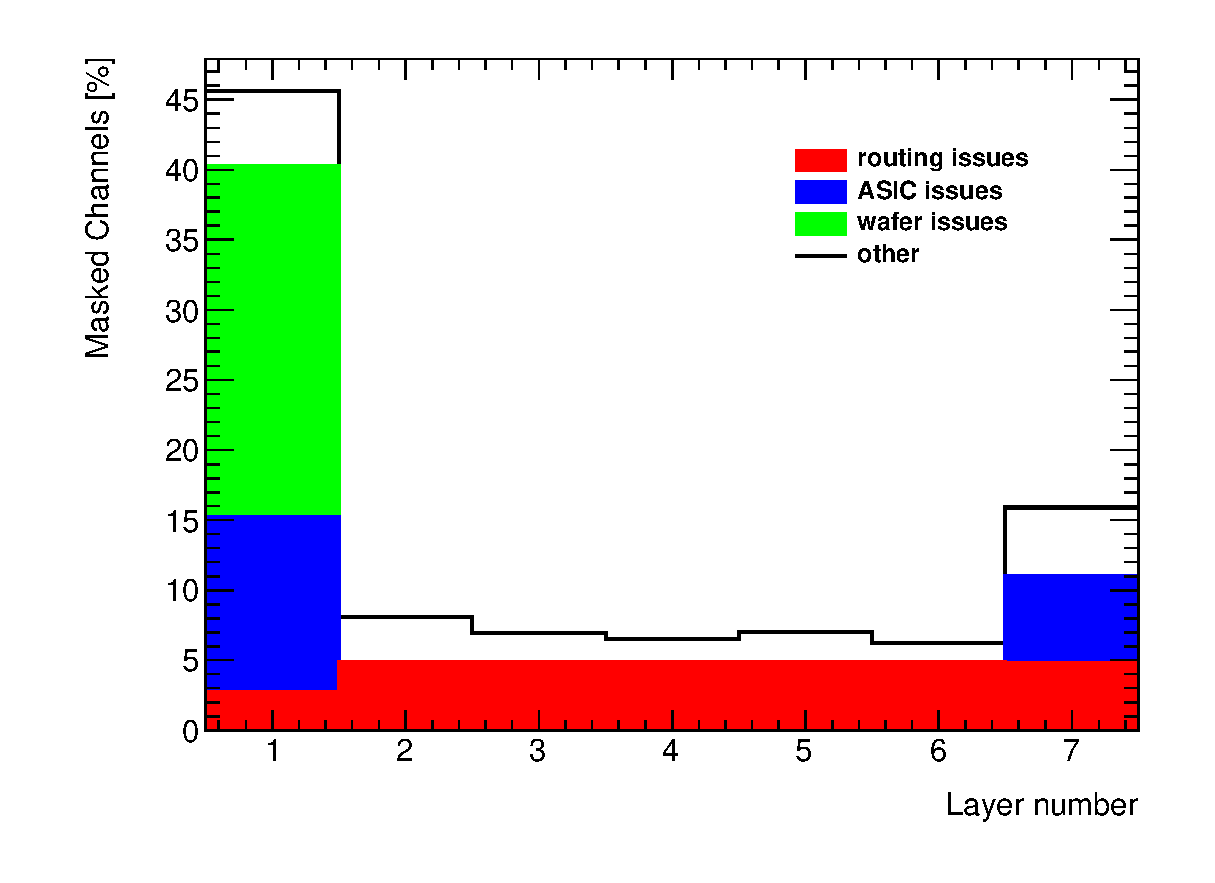
\includegraphics[width=4in]{figs/commissioning/masked_layer.eps} \\
  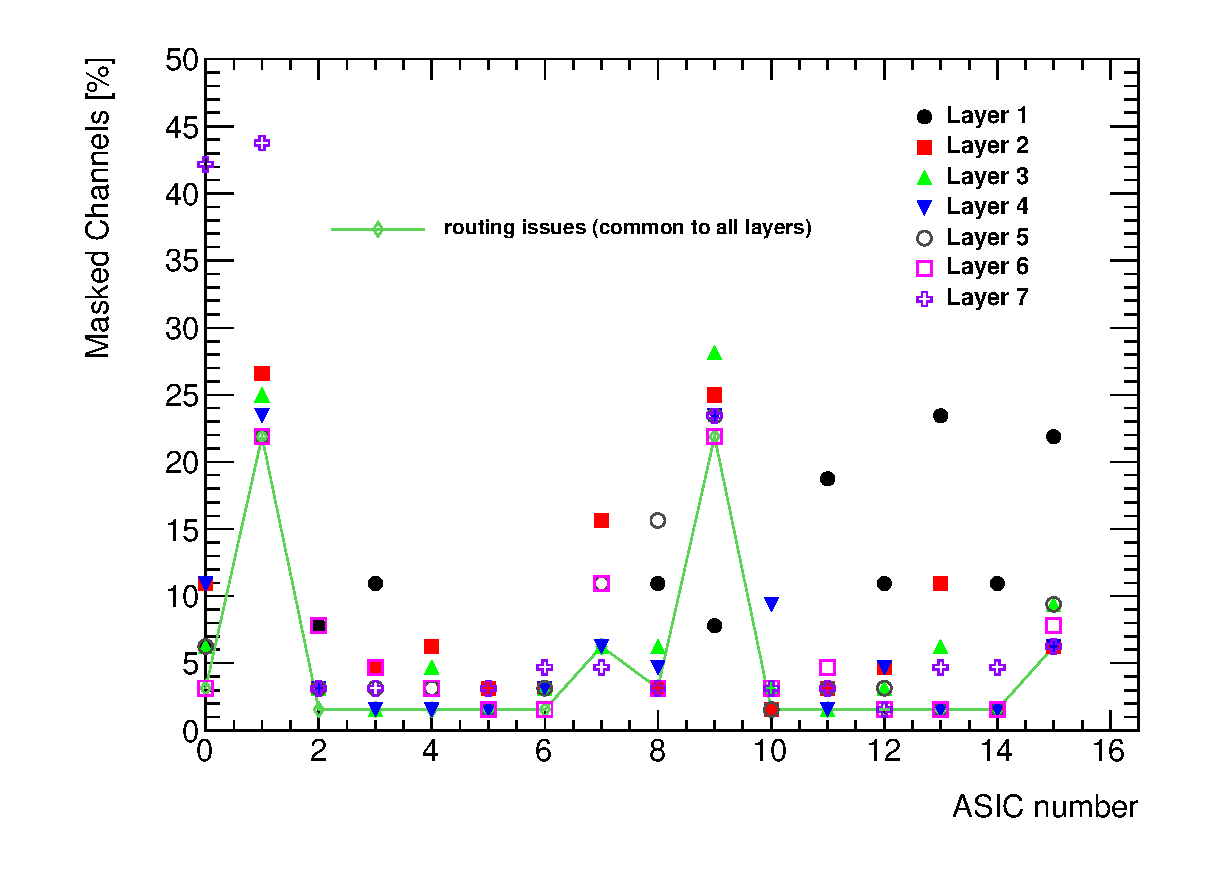
\includegraphics[width=4in]{figs/commissioning/masked_chip.eps}
  \end{tabular}
\caption{Ratio of channels that are marked as noisy in all slabs. 
Top: inventory of the different type of noisy channels per slab. 
Bottom: break up of the noisy channels per ASIC. We see two spikes in the number of channels masked due to routing issues in the ASICs 1 and 9. 
These two ASICs are located near the SMB where the density of lines (data and power transmission) is higher, complicating in this way the
routing. The ASICs 4-7 (wafer issue) and 10 from layer 1 and the ASIC 4 from layer 7 are not included
in the second plot since they are fully masked.}
\label{noisycells}
\end{figure}

We observed that the noise bursts happening coherently at the same time in all SLABS
was associated to cases when the electrical isolation between SLABs was broken.
This is a hint of a system effect as grounding loops or noise in the power supplies.
The issue was circumvented by improving the electrical isolation of single layers.
We have also observed that the noise burst happen only at the end of long acquisitions therefore, in addition to the improved isolation,
we selected short enough acquisitions windows (which indeed are the most appropriate to the high rates of particles in the DESY beam).
However, more studies in the laboratory are needed in order to fully understand these issues.

\subsection{Threshold determination}
\label{sec:comm_trigger}

Once that the SKIROC main settings have been fixed and the masking of the noisy channels at a relatively high threshold value
has been done, the final step is the selection of the optimal trigger threshold values.
For that, we perform dedicated runs in which we scan a reasonable range of trigger threshold values (in DAC units)
with all channels enabled (excepted the marked as noisy). For each of the DAC points
we took data during $\sim$ 1 minute per DAC in order to speed up the commissioning.
Plotting the total number of hits normalized to the maximum vs the DAC
for each channel gives the so-called S-curves. In the absence of external signals (cosmic rays, injected signals, etc) 
these noise S-curves show the convolution of the envelope of the 
electronic noise at the output of the fast shaper (the trigger decision line).
Indeed, the size of this enveloppe is related to slow clock frequency
(larger periods, larger possibility to find a noise variation over the threshold).

To reduce to the minimum the
presence of cosmic rays signals, we perform runs with short open acquisition windows (1.1 ms). 
In Figure \ref{scurve_channels} 
two S-curves of two different channels from the second layer of the setup are shown.

The S-curves are fitted to a complementary error function
\begin{equation}
S(DAC)=p_{0} \times erfc(\frac{DAC-p_{1}}{p_{2}}) = 
\newline
\frac{2p_{0}}{\sqrt(\pi)} \int_{\frac{DAC-p_{1}}{p_{2}}}^{\infty} \exp^{-t^{2}} dt,
\label{eq_S-curve}
\end{equation}
where $p_{0}$ is 1/2 of the normalization, $p_{1}$ is the value in which the noise levels are 
the 50\% of its maximum and $p_{2}$ give us the width of the S-curve. 

\begin{figure}[!t]
  \centering
  \begin{tabular}{ll}
  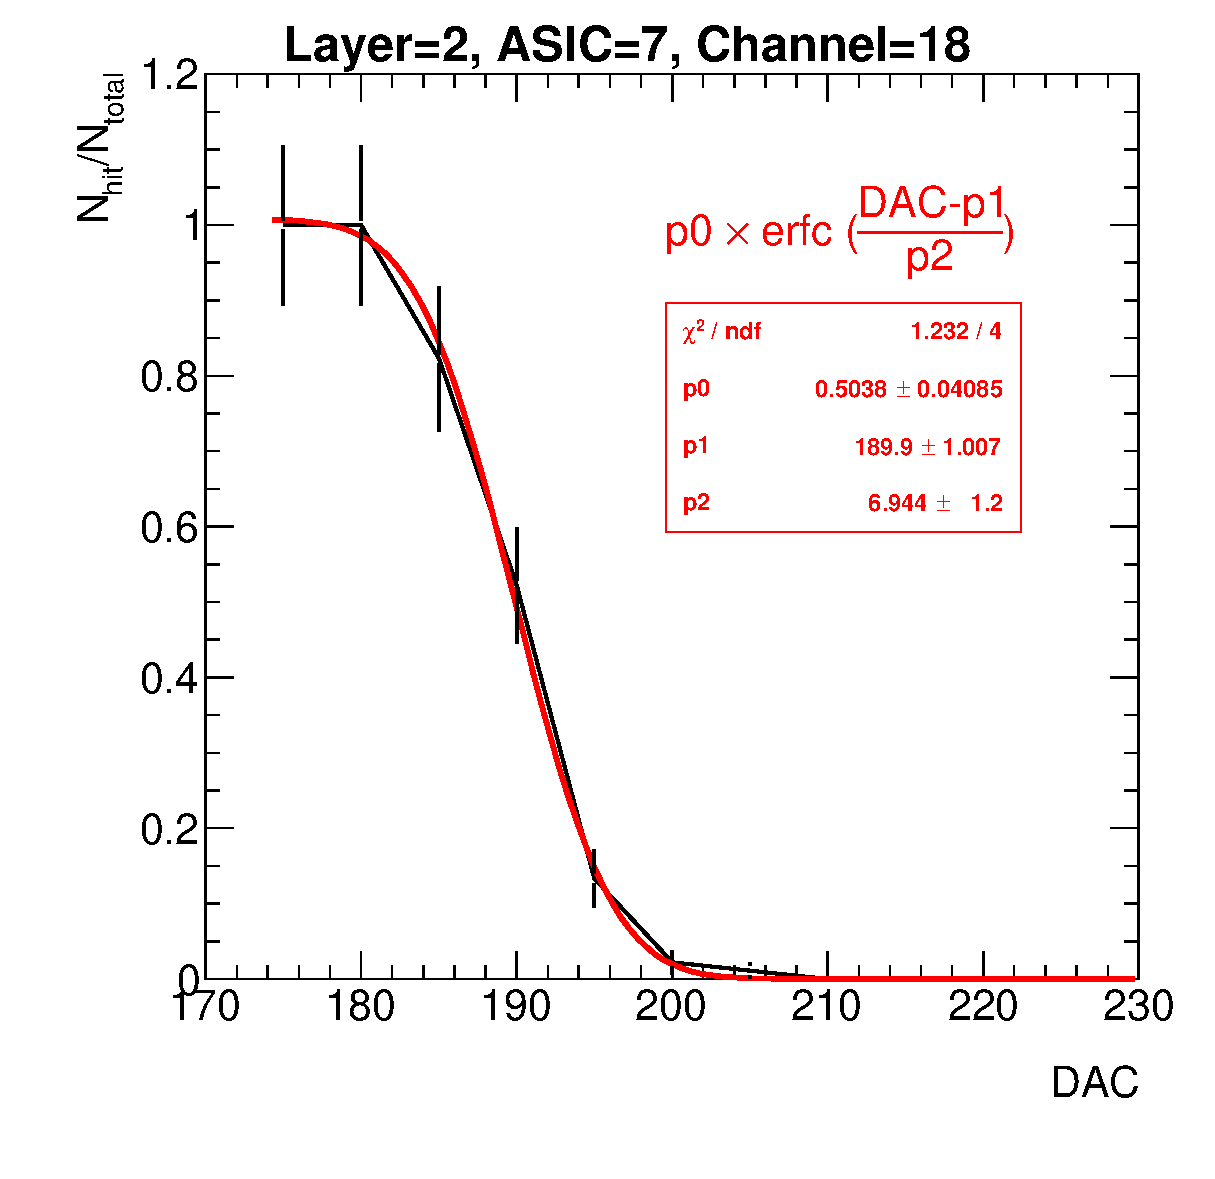
\includegraphics[width=2.8in]{figs/commissioning/scurve_chn18_asic7_layer2.eps} & 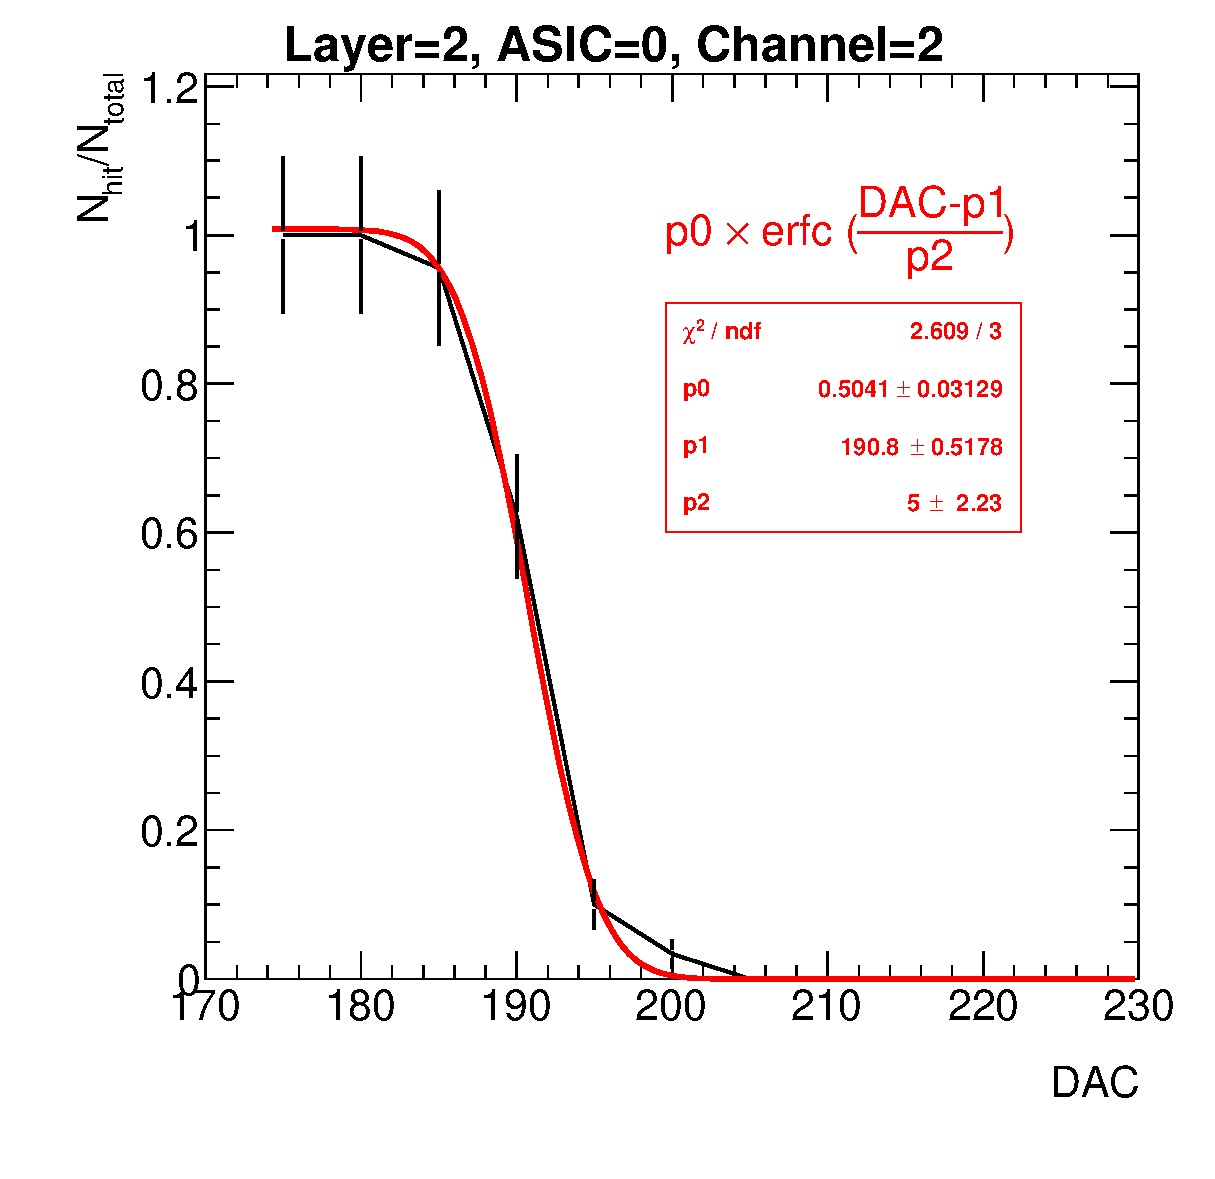
\includegraphics[width=2.8in]{figs/commissioning/scurve_chn2_asic0_layer2.eps}
  \end{tabular}
\caption{Two S-curves obtained during noise runs.}
\label{scurve_channels}
\end{figure}

The function from equation \ref{eq_S-curve} was fitted to all
channels data and all the values of $p_{1}$ and $p_{2}$ were saved.
To decide the final trigger threshold value for the full ASIC, we took the maximum between:

\begin{equation}
DAC_{optimal}^{ASIC-j} = <p_{1}^{ASIC-j}> + 5 \times <p_{2}^{ASIC-j}>
\end{equation}
and 230 if more than the 30\% of the 64 channels S-curves in the ASIC could be fitted. 
If not, we took a most conservative value of 250 DAC. The election of these two values was 
sustained by previous experiences, see for example \cite{Amjad:2014tha}.

The optimal trigger threshold values for all ASICs are shown in Figure \ref{trigger_thresholds}.


\subsection{S/N ratio in the trigger line}
\label{sec:comm_trigger_sn}

Similar kind of measurements can be done but using external signals. 
This will allow to calculate the signal over noise (S/N) ratio to trigger 1 MIP signals.
To calculate the S/N of the trigger we need to compare the 1 MIP S-curve and 2 MIP S-curve. The S/N 
will be defined as the ratio between the distance of both S-curves at its 50\% and the width of the 
S-curve.

In Figure \ref{scurves_injection} we see the 1 MIP and 2 MIP S-curves obtained for a one channel
in a SKIROC testboard in which a single SKIROC2 in BGA package is placed and the 1 MIP and 2 MIPs 
"fake" signals are directly injected in the preamplifier (via a 3 pF capacitor in the injection line). 
From this plot we can extract a S/N ratio of $\sim$12. 
We don expect large differences with the results that we would obtain with 
full equipped SLABs 
although this board is thought for commissioning and test of the SKIROC ASICS in an
"ideal" environment in contrast with the FEV
ASUS that are optimized to meet detector constraints and to hold several ASICs at the same time.
For example: only power pulsing of the analog power is done in this testboard,
there is a set of external capacitors on the board connected to some ASIC pins and
usually only one channel is tested. This allows us to commission the SKIROC2 itself

\begin{figure}[!t]
    \centering
  \begin{tabular}{l}
	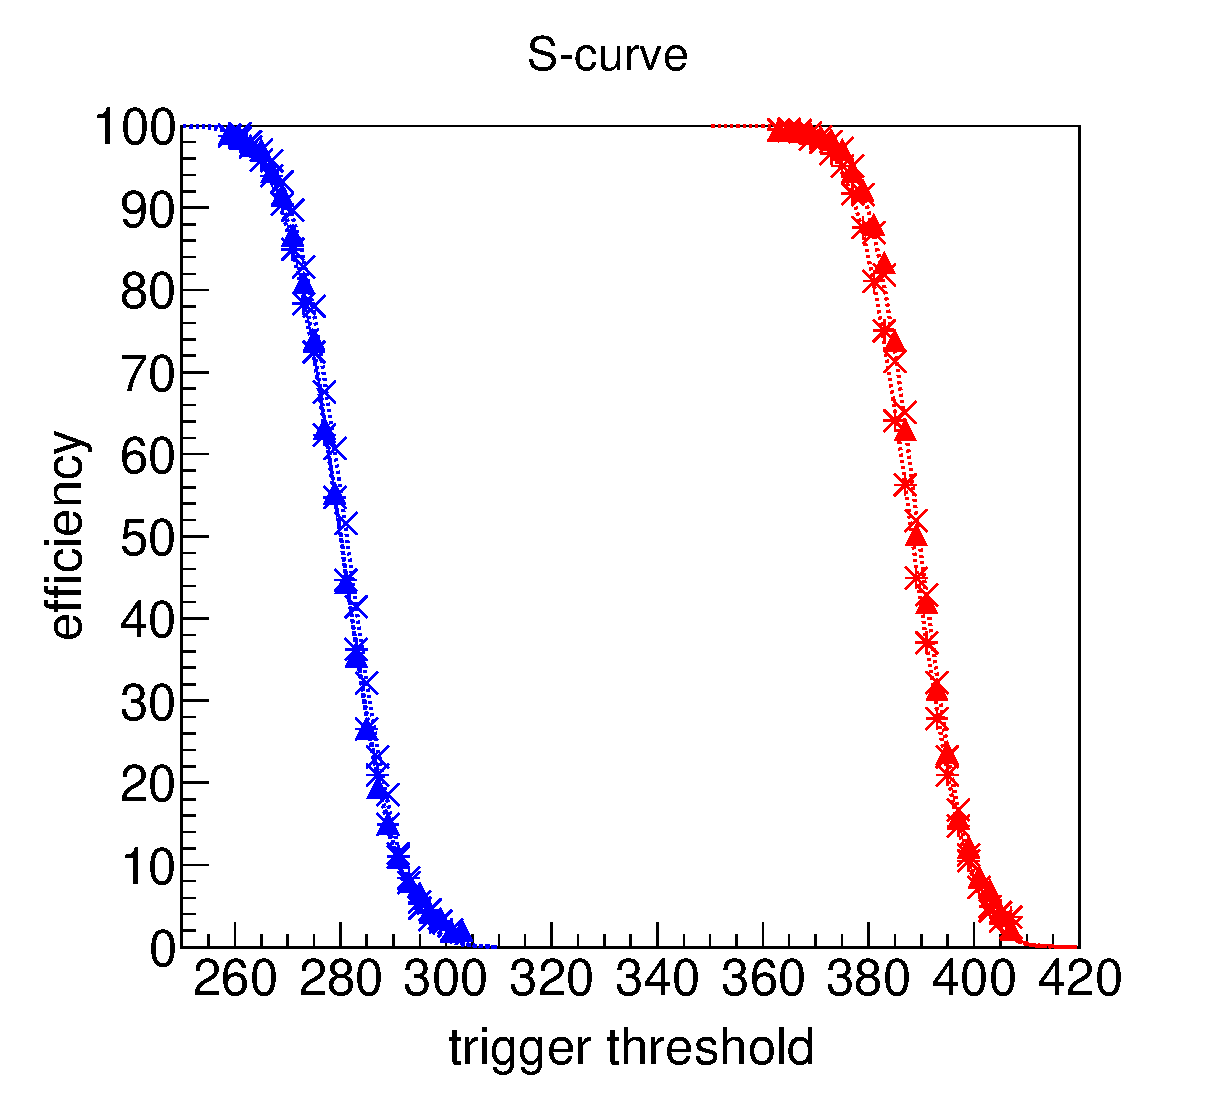
\includegraphics[width=4in]{figs/commissioning/scurve_pp_fastshaper_ch.eps} \\
	\end{tabular}
\caption{S-curves with charge injection (1 MIP in blue and 2 MIPs in red) for two different channels in a SKIROC2 testboard. From this plot, we extract a $S/N = 12.8$ in the trigger line.}
\label{scurves_injection}
\end{figure}


We have obtained similar results using real signals, in this case cosmic rays signals. This is shown 
in Figure \ref{scurves_cosmics}  where 
we show the result of the fit to the noise S-curves for all channels (in red) in one of the ASICs of 
the second layer together with the results of the S-curve with cosmic rays (black points and blue 
line). For the cosmic S-curve we took 30 min of data per point using very long spills (150 ms) in 
frequencies of 5Hz and we add up the triggers from all channels together. In addition, using the 
knowledge of the MIP value (see next section), we performed a simple cut in the ADC
to keep only signals corresponding to a MIP 
(pedestal subtracted) $\pm30$ ADC counts. With this cut we try reduce the contribution of muons 
traversing the wafers with very large angles but we don't have a way to select perpendicular tracks 
since we were using simple setups with only single slabs during in the run. For all these reasons, we expect
a broader distribution of the cosmic S-curve. This is one of the reasons why, if we calculate the S/N 
using this plot, the value would be unrealistic (much lower, indeed). 
In addition to this, we should remember that the noise S-curve do correspond to the real noise 
distribution but only to the envelope of the noise in the fast shaper, therefore the
distance between the two S-curves is smaller than the real distance between noise and signal.

\begin{figure}[!t]
    \centering
  \begin{tabular}{l}
	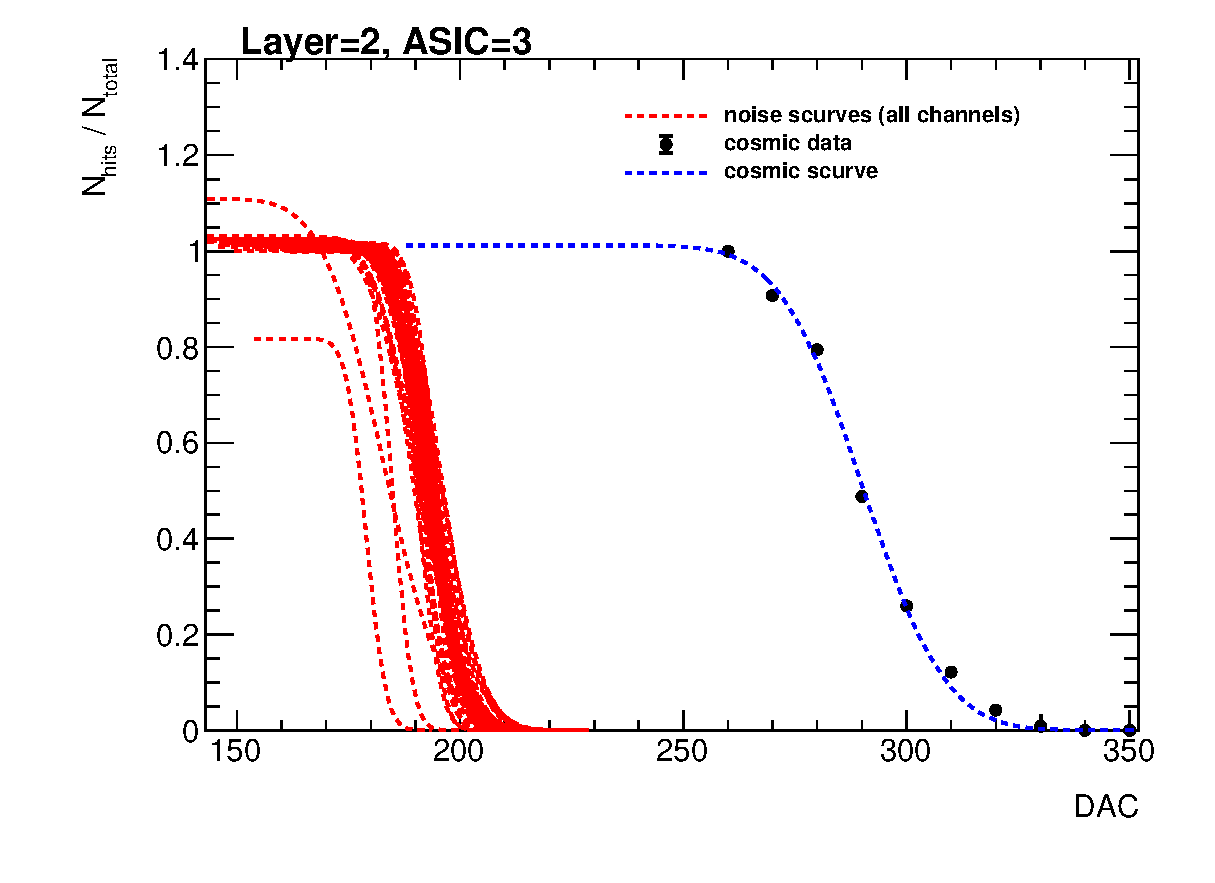
\includegraphics[width=4in]{figs/commissioning/cosmic_scurves_asic3_layer2.eps} 
	\end{tabular}
\caption{S-curves for noise (channel by channel, only the result of the fit) and cosmic rays (all channels together) for one ASIC in layer 2.}
\label{scurves_cosmics}
\end{figure}

In conclusion, both ways of estimating the S/N ratio of the trigger have their own limitations but in 
both cases, the 50\% of the S-curve of 1 MIP are compatible within $\pm10$ ADC. This allow us
to, at least, estimate the relative distance between our final trigger threshold for every ASIC and 
the 1 MIP position. This is shown in Figure \ref{trigger_thresholds}. Two ASICS ($\sim2\%$) have a
trigger threshold value of 0.67 MIP. The 11\% of the ASICs have a trigger threshold between 0.5 and 0.55 MIP and the rest, 87\%, have trigger thresholds slightly lower 0.5 MIP.

\begin{figure}[!t]
  \centering
  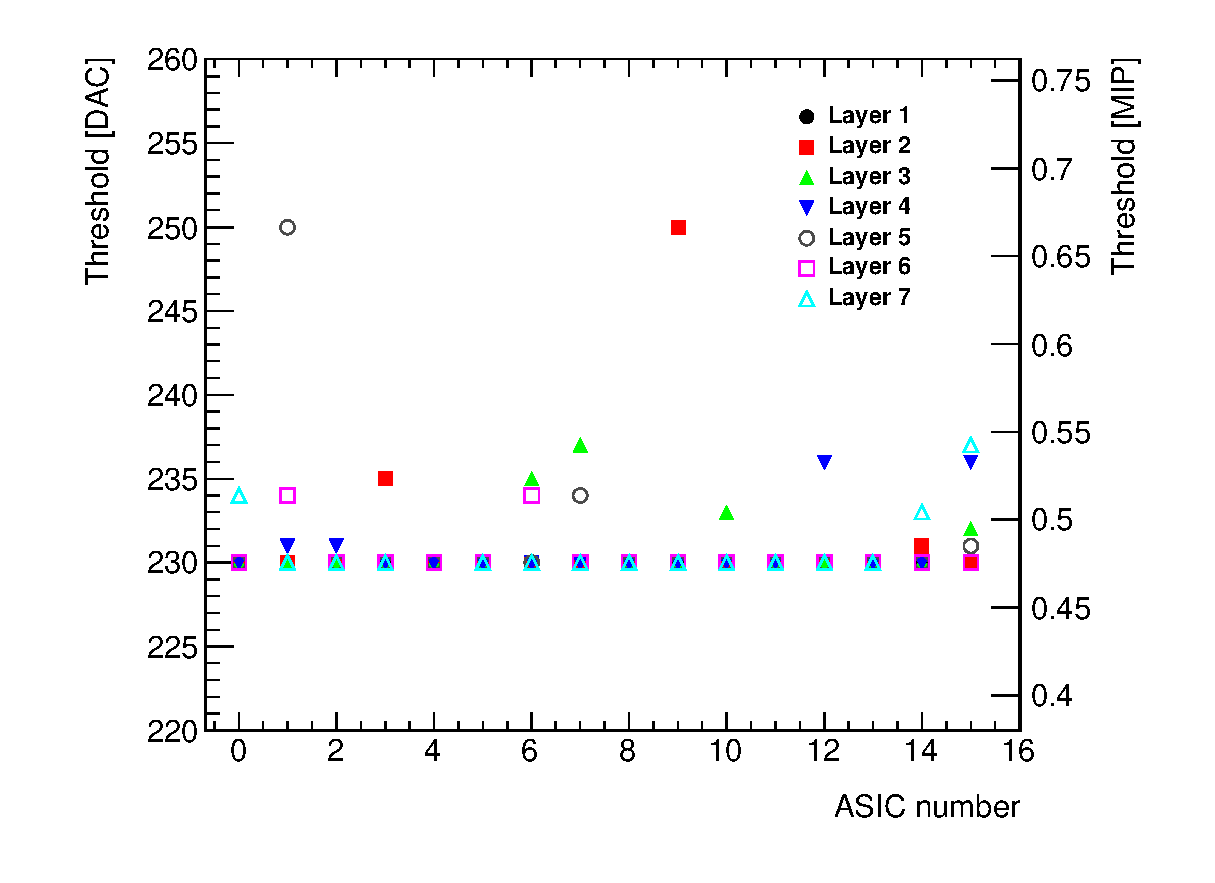
\includegraphics[width=4in]{figs/commissioning/threshold_chip.eps}
  \caption{Summary of trigger threshold settings for all ASICs in the setup. The values are given in DAC and in estimated MIP units, using the distance between two MIPs from Figure \ref{scurves_injection}. The uncertainty quoted in the right axis is estimated from difference between the 50\% position of the S-curve for one MIP extracted from this figure and Figure \ref{scurves_cosmics}.}
\label{trigger_thresholds}
\end{figure}


\subsection{Prospects}
\label{sec:comm_prospects}

All the commissioning procedure described above relies in very conservative decisions
due to the presence of unknown noise sources during most of the commissioning phase. These sources are
now well know and isolated and therefore a new ``noise'' commissioning procedure can proposed
for the next beam test. It will consist in an iterative algorithm that first
will identify and mask the "underflowed-noisy" channels and afterwards run a set of acquisitions
in which the number of triggers per channel will be compared with the number of expected triggers
assuming only cosmics rays as signal. This will allow us to have an
unambiguous definition of the noise levels channel per channel instead of 
defining that levels relatively to the total number
of recorded triggers. Finally, once that the noisy channels
are identified, the optimization of the threshold levels
will be performed and the last run for identification of noisy channels will be taken using this optimal
level will be taken. In this run, we can decide to mask the noisy channels or
to increase its own trigger threshold level if we are using Skiroc2a.

Using this new procedure we manage to reduce the number of masked channels by a factor 2 without any loss of performance,
at least in the laboratory and using 3 of the 7 SLABs. This new procedure will be tested in the next beam test.
Also, in order to
optimize the commissioning of the detector,
we will propose a new set of measurements in the next beam test consisting in:
a scan of optimal delay of the hold values of the trigger using MIP like particles;
and a threshold scan for the determination of the S/N in the trigger line using
1 MIP and $\sqrt{2}$ MIP (tilting the detector by 45 degrees) signals.


\section{Performance on positron beam test at DESY}
\label{sec:beamtest}


The beam test line at DESY provides continuous positron beams in the energy range of 1 to 6 GeV with
rates from few hundreds of Hz to few KHz with a maximum of $\sim 3$ KHz for 2-3 GeV. 
These positrons are produced in the following way: first, the electron/positron synchrotron DORIS II 
is used to produced a photon beam via bremsstralhung when interacting with a carbon fiber target;
secondly, these photons are then converted to electron/positron pairs; 
and, finally, the beam energy is selected with dipole magnets and collimators. 
In addition, DESY gives acces to a bore 1 T solenoid, the PCMag.

The prototype tested in beam in June 2017 consisted of 7 layers as explained in Section \ref{sec:setup}.
The detector was exposed to a positron beam in the DESY test beam area (line 24).
By means of an external pulse generator we defined the length of the acquisition window to be
3.7 ms at a frequency of 5 Hz, emulating in this way similar conditions than the ILC will have.
The detector was running in power pulsing mode without any extra active cooling system.

The physics program of the beam test can be summarized in the following points:

\begin{itemize}
\item Commissioning and calibration without tungsten absorber using 3 GeV positrons acting as minimum ionizing particle (MIPs);
\item magnetic field tests up to 1 T in the PCMag;
\item response to electrons with fully equipped detector, i.e. sensitive parts {\it and} W absorber.
\end{itemize}

For the first two points from above, we used the SiW-ECAL in the tracker mode, {\it i.e.} without 
intercalated tungsten plates. Due to the low material budget of our setup when the tungsten is not 
included, a beam of positrons of few GeV of energies provides satisfactory data for calibration since 
the positrons deposit the minimum amount of energy by ionization.
The calibration of the detector was realized 
by directing the 3 GeV positron beam on 81 positions equally distributed over the surface of the 
detector.
These data were used for pedestal estimation and energy calibration.
Calibration and pedestal analysis was done for all single layers not requiring track reconstruction.
The study of these data is discussed in Section \ref{sec:pedestal} for the pedestal and noise studies and Section \ref{sec:mip} for the results of the calibration.

For the tests inside the magnetic field, a special PVC structure was
designed and produced to support one single SLAB.
The purpose of such test was twofold: first to prove that the DAQ, all electronic devices and the 
mechanical slab itself were able
to handle strong magnetic fields; second to prove the stability of the performance during these tests.
We took several runs, with 0, 0.5 and 1 T magnetic fields with and without 3 GeV positron beam and 
we observed that the pedestal and noise values are independent of the magnetic field (see Section 
\ref{sec:magnetic}). The study of the MIP calibration stability will be discussed in future 
publications, where full studies of the data including comparison with simulations should be included.

To fulfill the last point of the list we inserted W plates of different thicknesses between the 
sensitive layers. Then we performed
a scan of energies of the positron beam: 1-5.8 GeV.
We tested the response of the detector with three different configurations of the W repartition.
The accumulated amount of tungsten, in radiation length units, $X_{0}$, in front of each of the 
SLABs is:
\begin{itemize}
\item W-configuration 1: $0.6,1.2,1.8,2.4,3.6,4.8$ and $6.6~X_{0}$
\item W-configuration 2: $1.2,1.8,2.4,3.6,4.8,6.6$ and $8.4~X_{0}$
\item W-configuration 3: $1.8,2.4,3.6,4.8,6.6,8.4$ and $10.2~X_{0}$
\end{itemize}

Preliminary results of the raw electromagnetic shower profiles look promising but will not be 
discussed in this article since deeper analysis and comparison with montecarlo simulations
will be needed to extract conclusive results from the data. This will be the topic of a future 
article, possibly combining data with future beam tests that are currently in preparation. What it
is included in this article, in Section \ref{sec:showers} is the study of the pedestals in this events.


\subsection{Pedestal and noise studies with the SiW-ECAL in tracker mode}
\label{sec:pedestal}

Due to the way that the SKIROC2 ASICs work, it is possible to extract the pedestals
simultaneously to the recording of signals from particle interactions. Indeed, when a channel
is triggered, the rest are read out at the end of the slow clock period (usually called BCID - for bunch crossing ID  and marked as
non triggered channels. This allows us to reconstruct the pedestal distribution
for all channels and for all SCAs. These distributions are fitted with a Gaussian
and the pedestal value are associated with the mean of the result of the fit.
These values will be, afterwards, subtracted to the ADC recorded by the SKIROC2 for all channels and SCAs.
The noise of the channel and SCA corresponds to the width of the pedestal distribution.
The calibration runs have been used to calculate the pedestal distribution reference values of the detector.
In Figure \ref{signal_pedestal} we show the signal and pedestal distribution of a single channel after
subtracting the pedestal mean position.

\begin{figure}[!t]
  \centering
  \begin{tabular}{l}
    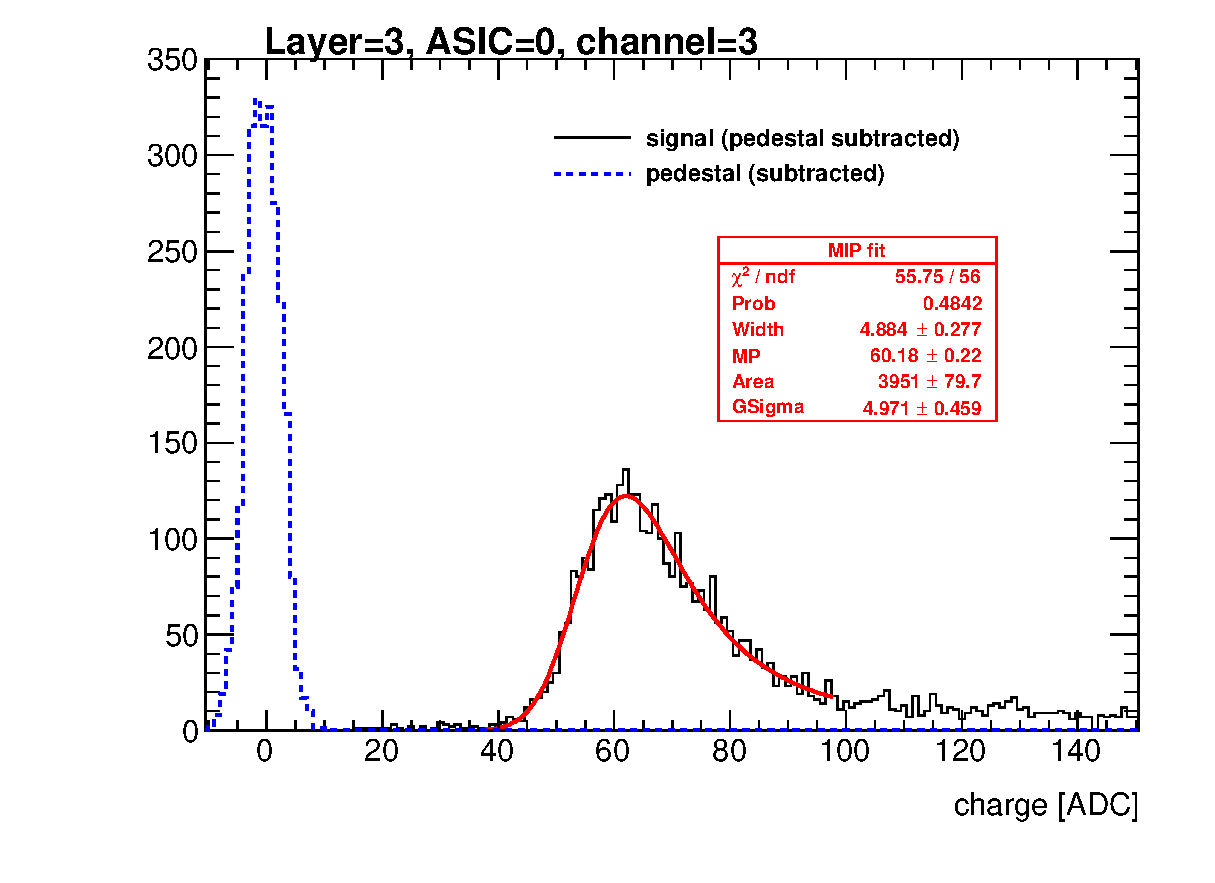
\includegraphics[width=4in]{figs/mip_pedestal_example.eps}
  \end{tabular}
  \caption{Pedestal (blue dashed line) and signal (black continuous line) distribution for one channel in the third layer. The results of the MIP calibration fit are included (red). The pedestal distribution is shown only for the first SCA to keep the y-axis within a reasonable range. The signal distribution is integrated over all SCAs.}
\label{signal_pedestal}
\end{figure}


In Figure \ref{pedestal_channel} (left) we observe that both the pedestal position for each SCA in the same channel can be
different in few \%s. In the case of the pedestal mean position, these differences are even larger between different ASICs in the same
layer (Figure \ref{pedestal_layer}, left plot) or between layers (Figure \ref{pedestal_all}, left). This is the reason of
performing the pedestal correction layer-, chip-, channel- and SCA-wisely.
For the noise, the dispersion is smaller ($\sim 5 \%$) and only dependent on the SCA. This is shown in the right plots of Figures \ref{pedestal_channel}, \ref{pedestal_layer} and \ref{pedestal_all}.

\begin{figure}[!t]
  \centering
  \begin{tabular}{ll}
    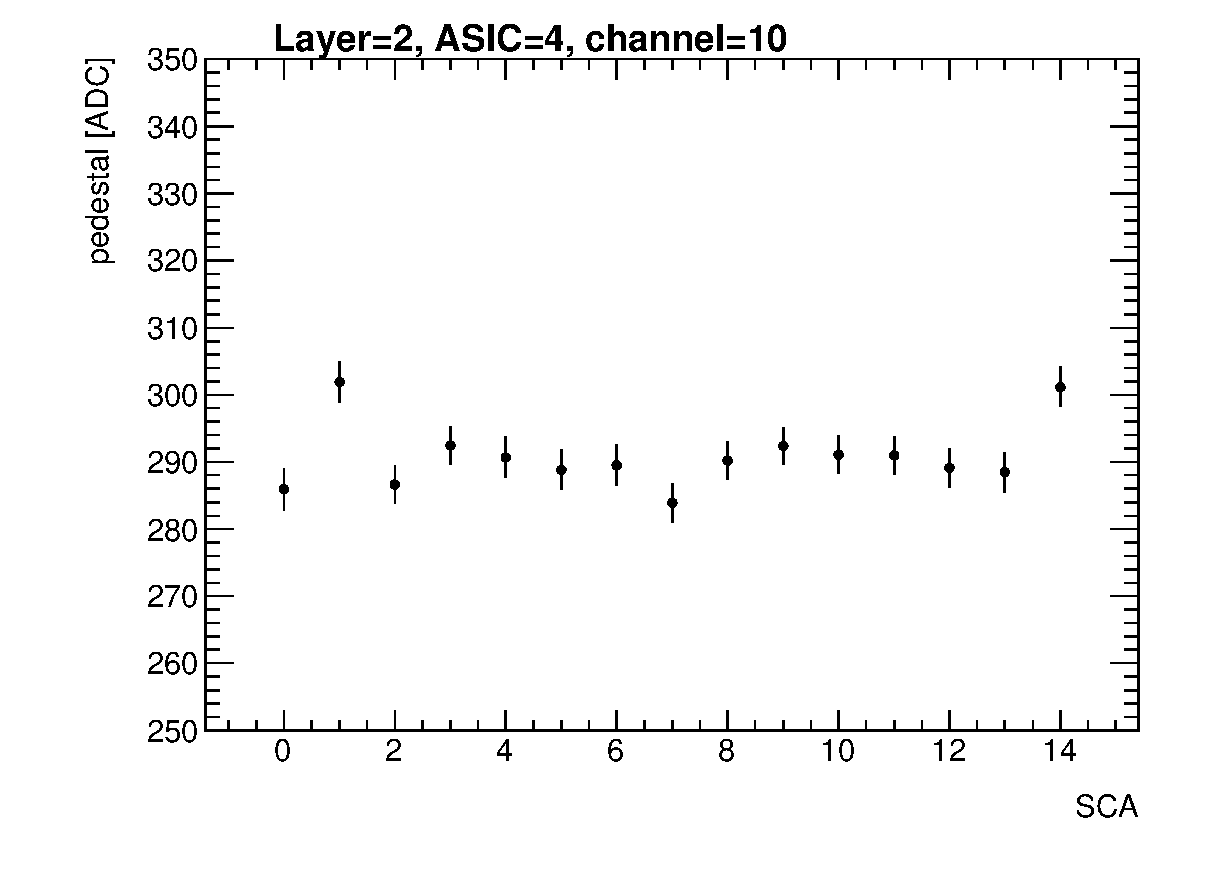
\includegraphics[width=2.8in]{figs/pedestal/ped_mean_layer2_chip4_cell10.eps} & 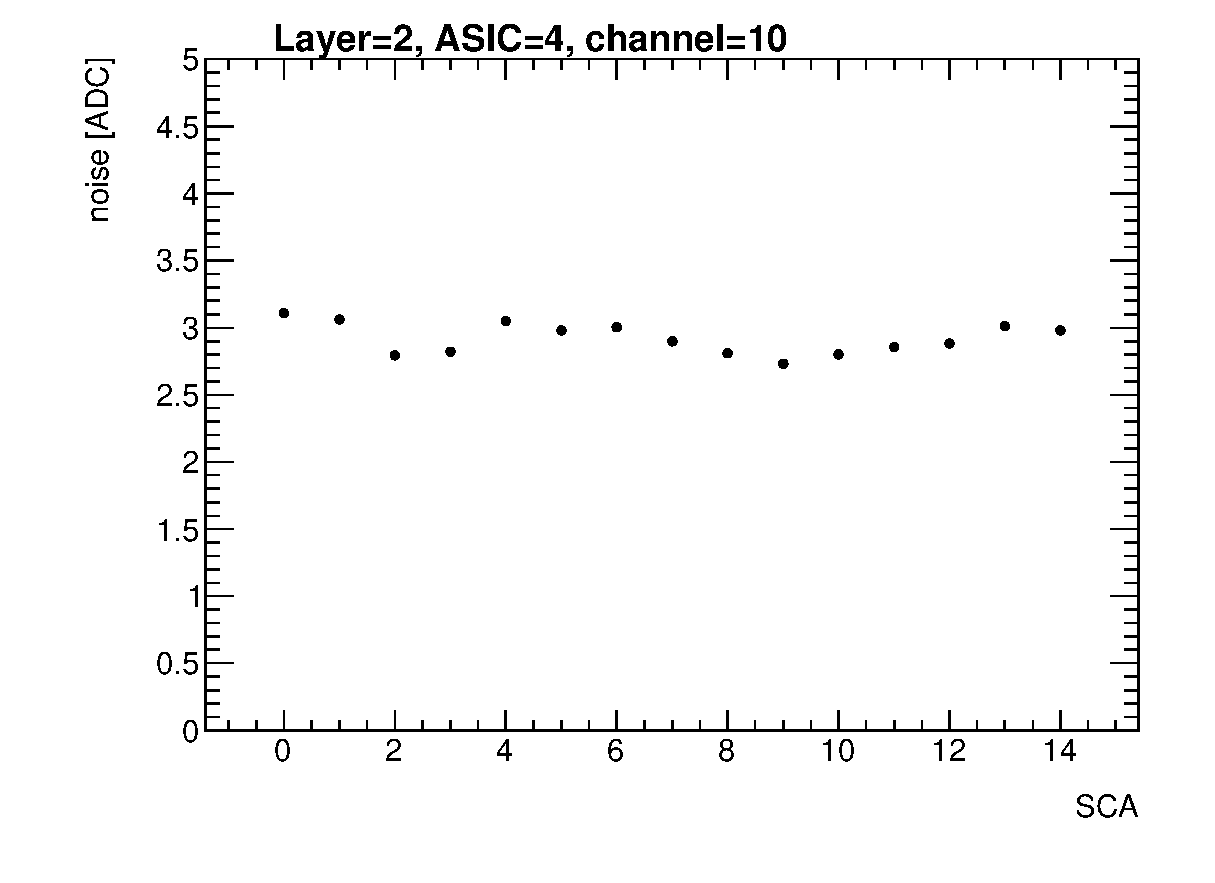
\includegraphics[width=2.8in]{figs/pedestal/ped_width_layer2_chip4_cell10.eps}
  \end{tabular}
  \caption{Pedestal mean position (left) and width (right) for one channel in the second layer.}
\label{pedestal_channel}
\end{figure}

\begin{figure}[!t]
  \centering
  \begin{tabular}{ll}
    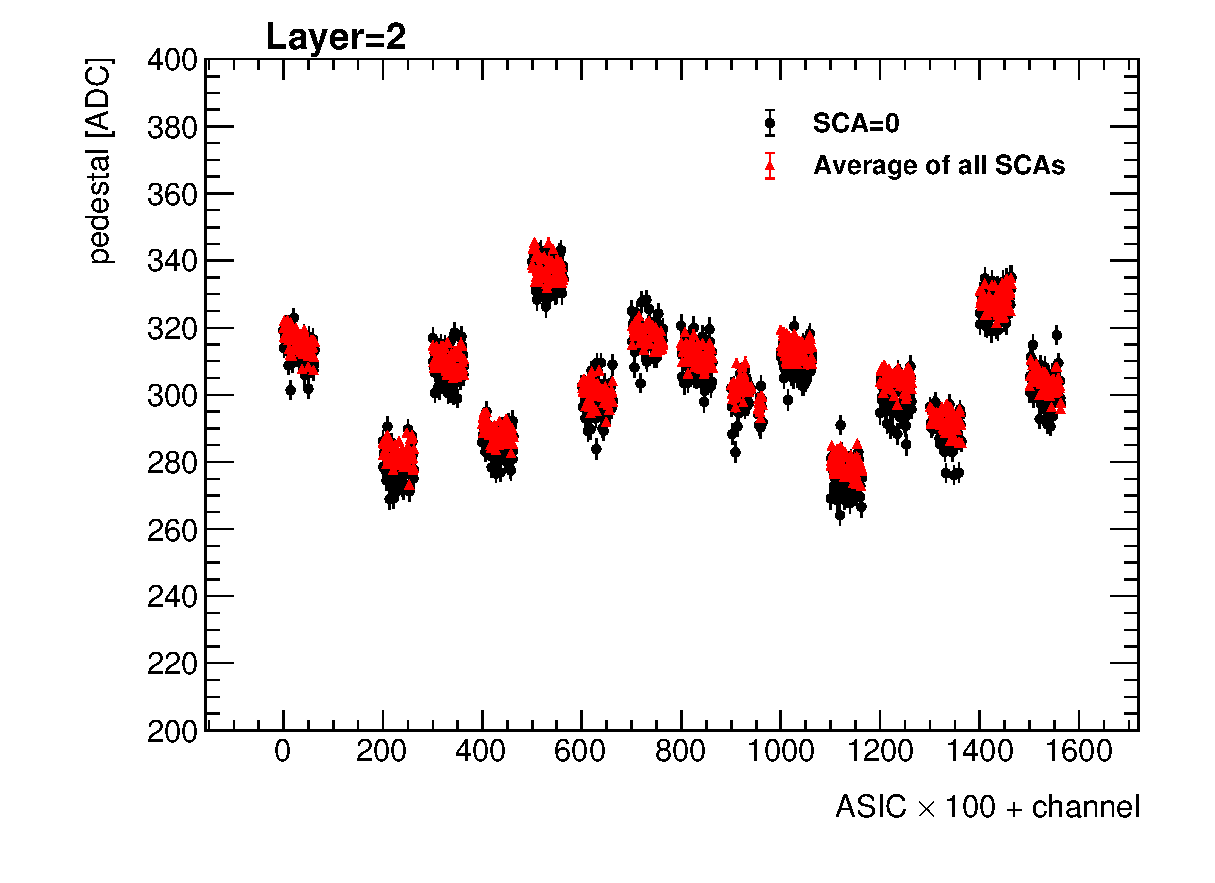
\includegraphics[width=2.8in]{figs/pedestal/ped_mean_layer2.eps} & 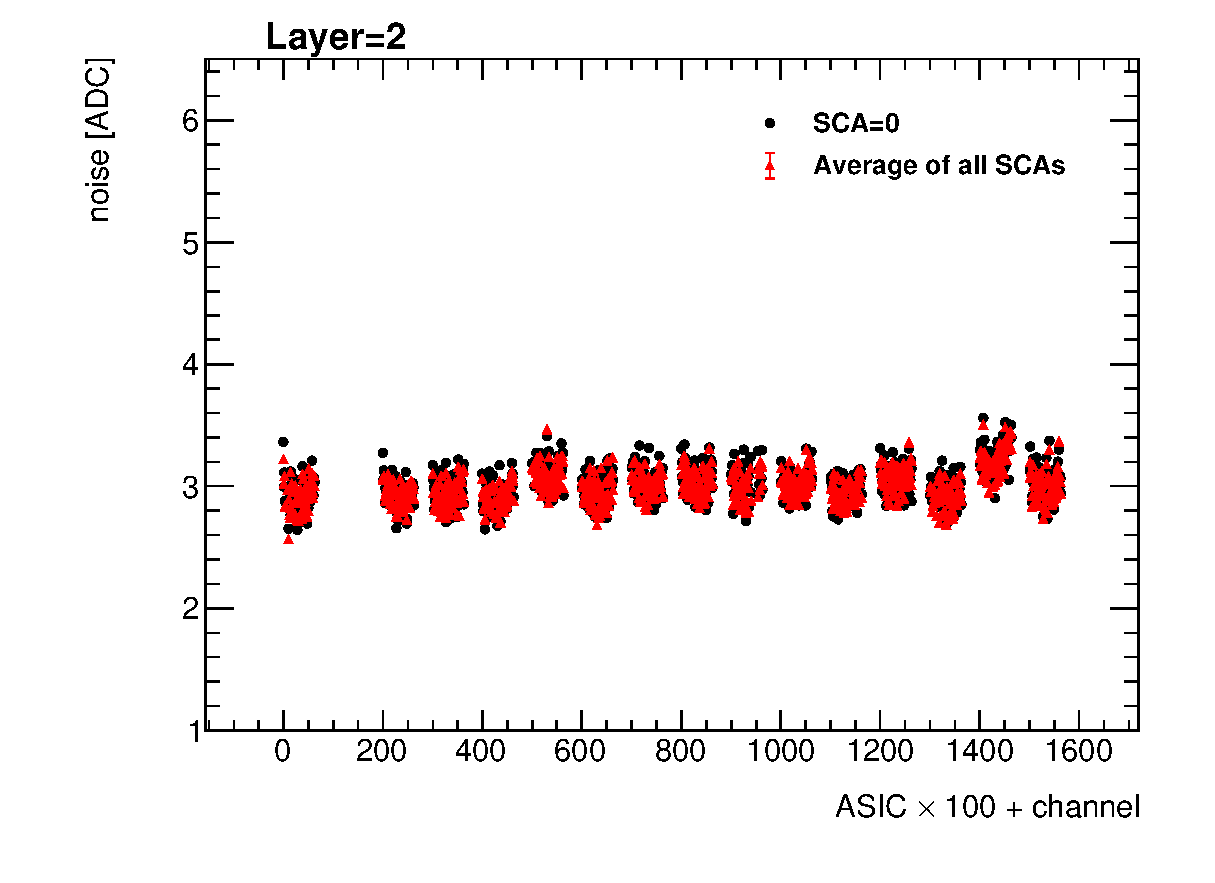
\includegraphics[width=2.8in]{figs/pedestal/width_mean_layer2.eps}
  \end{tabular}
  \caption{Pedestal mean position (upper plot) and width (lower plot) for all channels in one layer. The data is grouped on bunches in which the value in the x-axis
    corresponds to the value of the channel number plus the value of the ASIC number multiplied by 100. The black points show the value for the first SCA
    and the red points show the average value for all the others SCAs (with the standard deviation of the sample as error bar).}
\label{pedestal_layer}
\end{figure}

\begin{figure}[!t]
  \centering
  \begin{tabular}{ll}
    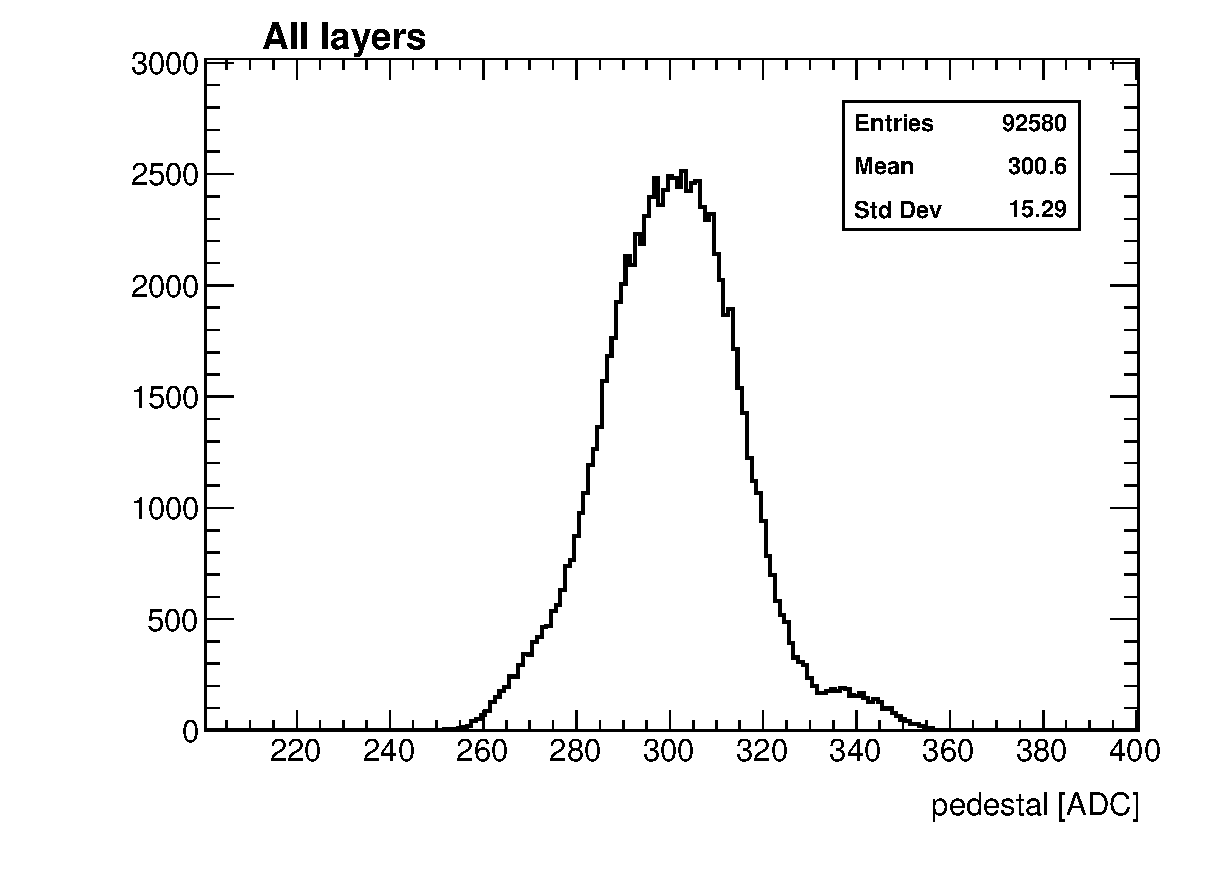
\includegraphics[width=2.8in]{figs/pedestal/h_ped_mean.eps} & 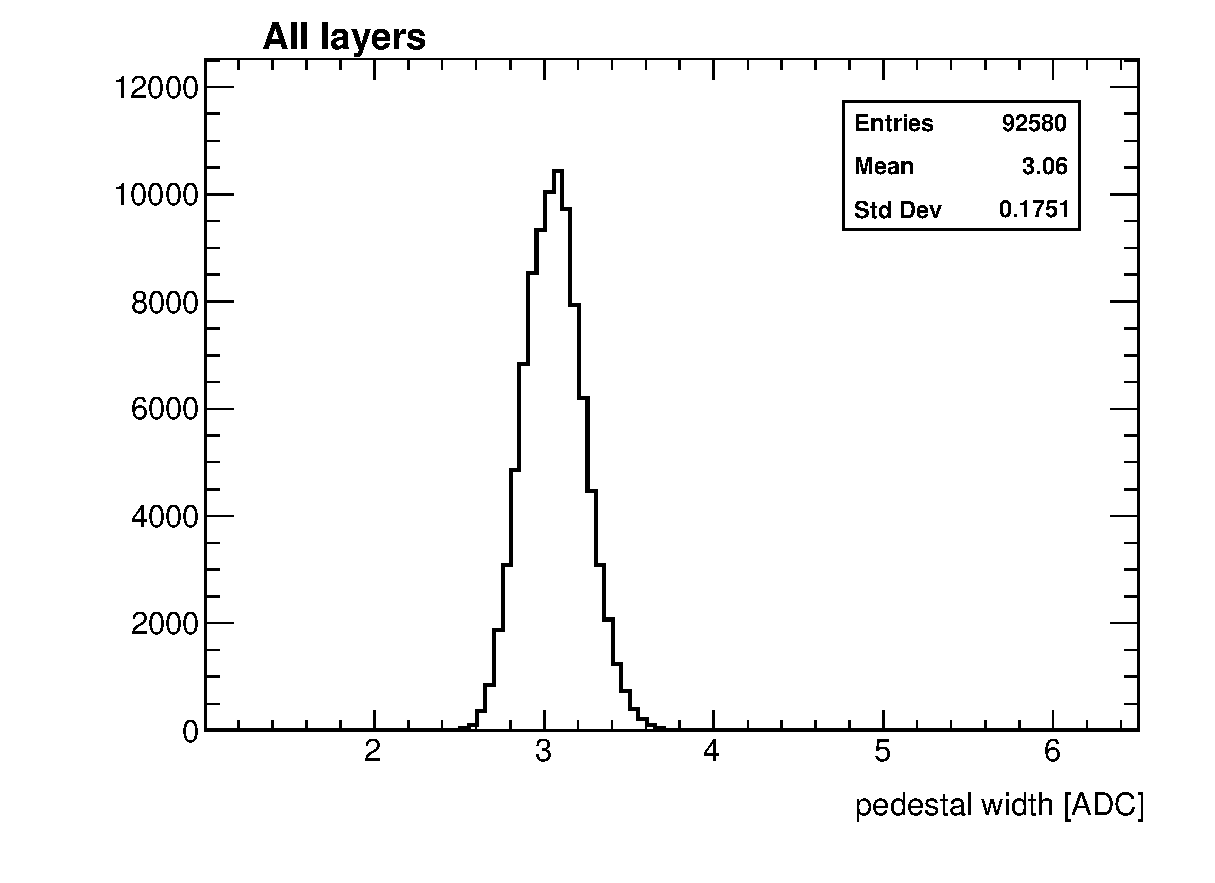
\includegraphics[width=2.8in]{figs/pedestal/h_ped_width.eps}
  \end{tabular}
  \caption{Pedestal mean position (left) and width (right) for all channels and all SCAs in the setup.}
\label{pedestal_all}
\end{figure}

\subsubsection{Pedestal and noise in large magnetic fields}
\label{sec:magnetic}

For the tests inside the magnetic field we used the SLAB of the first layer
in the special PVC struture mentioned at the begining of this section. We should also mention that
the PCMag is in a different area (downstream) on the same beam line,
therefore, due to the presence of additional collimators the beam rates are lower.

We divided the
data taking in 3 stages in this order:
a long run (13h) with a magnetic field of 1 T, a second and shorter run of 3 hours with 0.5 T and a final run with the magnet off.
In the cases were we had beam, we used the 3 GeV positron beam settings impacting in the ASIC number 12.

The comparison of the pedestal values and noise levels between the reference run in the stack
and the different runs in the magnetic field are shown in Figure \ref{pedestal_magnetic}.
We see that in both cases, the agreement is perfect within the statistical uncertainties.
Due to the lower rates in this beam area, the
analysis is only done up to few SCAs.

\begin{figure}[!t]
  \centering
  \begin{tabular}{ll}
    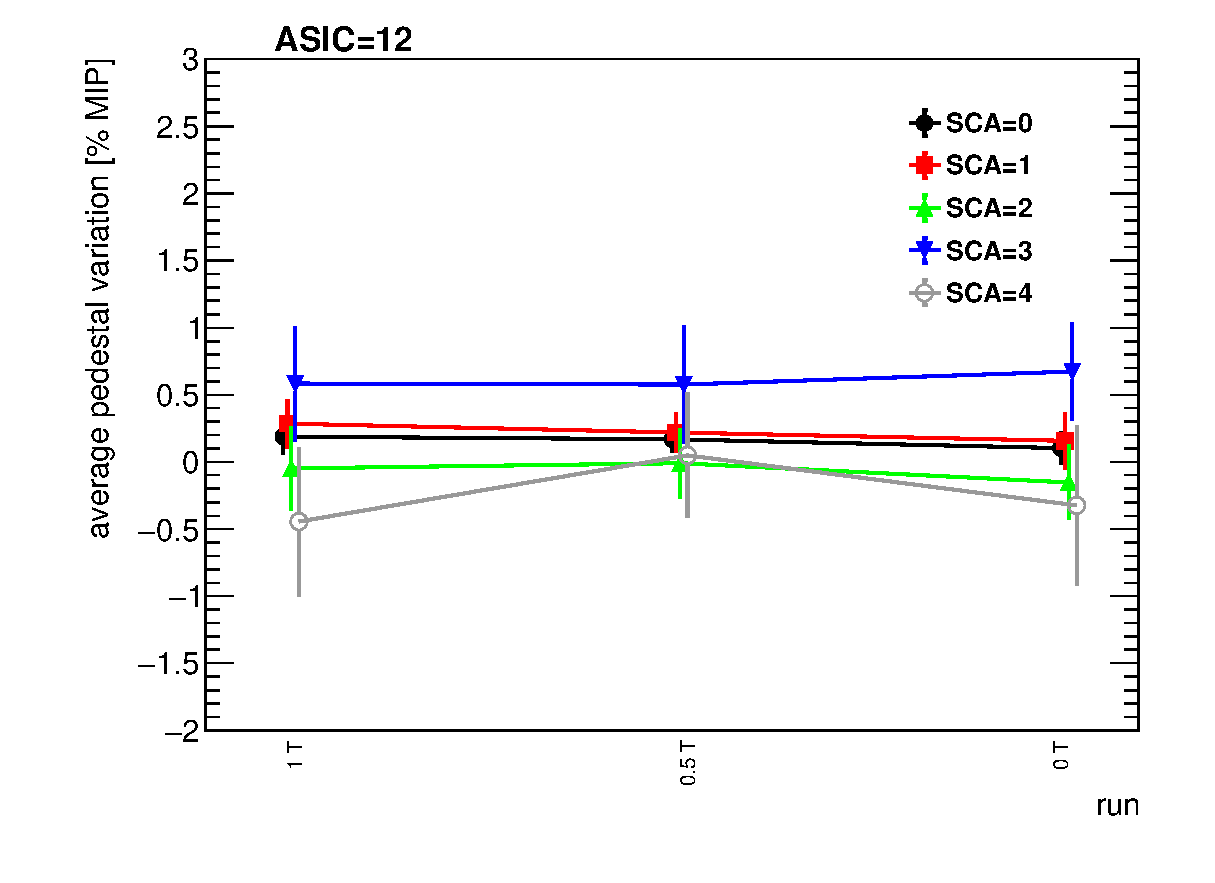
\includegraphics[width=2.8in]{figs/pedestal/1T/summary_pedestal_chip12.eps} & 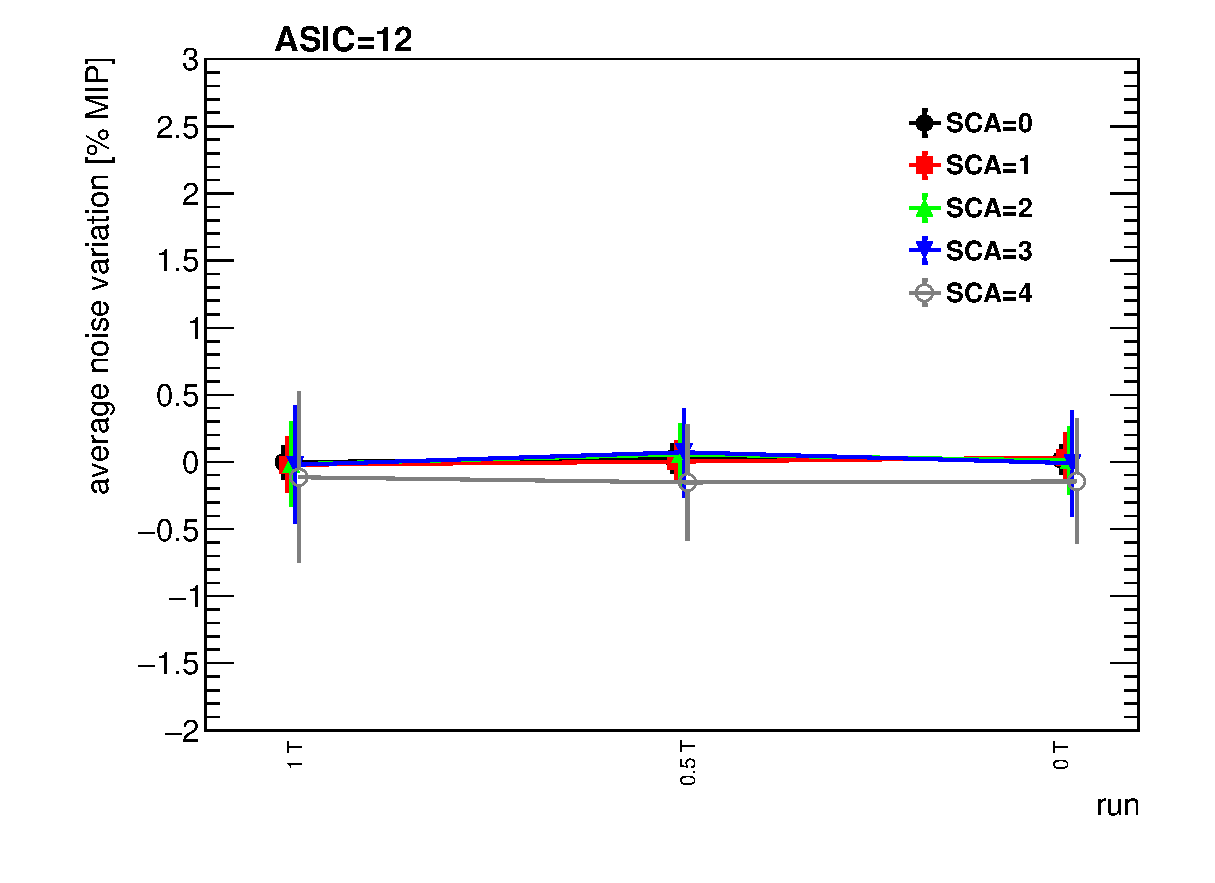
\includegraphics[width=2.8in]{figs/pedestal/1T/summary_noise_chip12.eps}
  \end{tabular}
  \caption{Average deviation of the pedestal mean position (left) and width (right) for all channels in the ASIC 12. The values are given in MIP units obtained from calibration (see Section \ref{sec:mip}).}
\label{pedestal_magnetic}
\end{figure}

\subsection{MIP response and tracking efficiency with the SiW-ECAL in tracker mode}
\label{sec:mip}

\begin{figure}[!t]
  \centering
  \begin{tabular}{ll}
      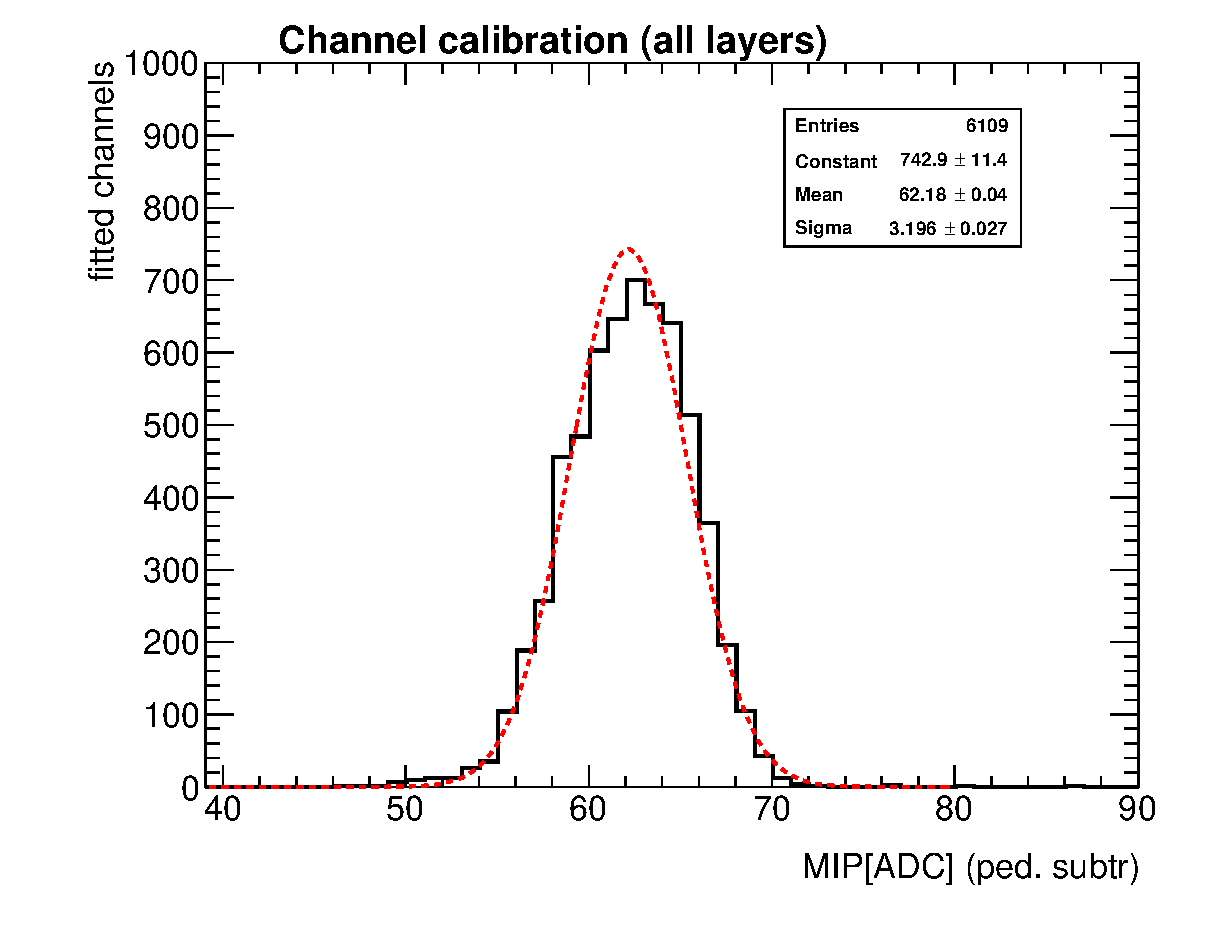
\includegraphics[width=2.8in]{figs/MIP/MIPsummary_title.eps} & 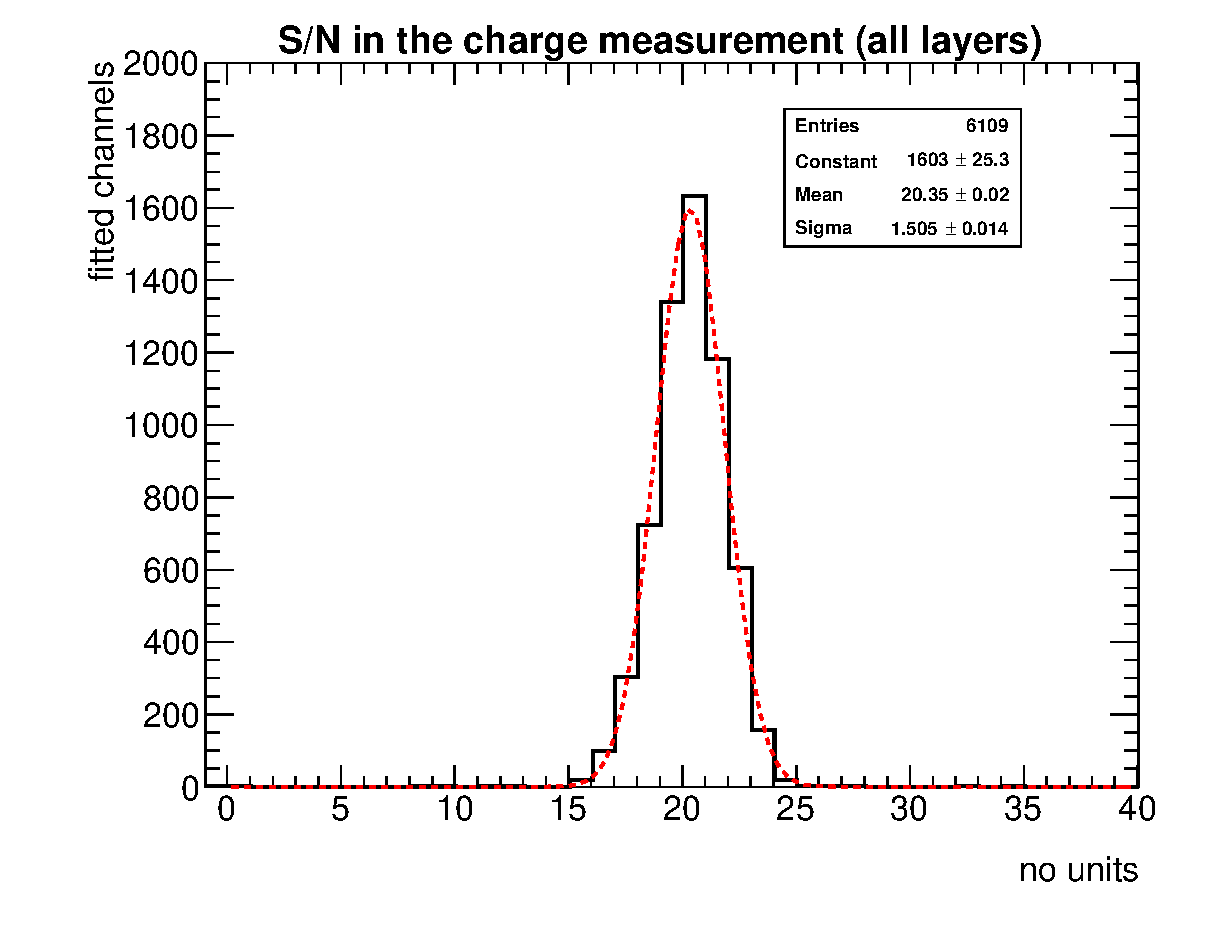
\includegraphics[width=2.8in]{figs/MIP/SNsummary_title.eps}  
  \end{tabular}
\caption{Result of the MIP position calculation and signal over noise calculation for all calibrated channels.}
\label{mipandSN}
\end{figure}
  

After the calculation of the pedestals for each channels and SCA, these are subtracted and the same data (without track
recognision) are used for the calibration.
A Landau function convoluted by a Gaussian is fit to the resulting hit distribution
in ADC units.
The most-probable-value of the convoluted function is taken as the MIP value, allowing thus for a direct
conversion from ADC to energy.
We have obtained a raw energy calibration spread of the 5\% among all channels with the 98\% of all 
available channels being fitted. Results are summarized in figure \ref{mipandSN}, leftmost plot.

We checked the MIP 
calibration by selecting tracks that cross the detector parallel to its normal
and filling a histogram with the energy measured by each channel with a hit.
We did this for all calibration runs together.
The results are shown in figure \ref{mip3peaks} where the single channel energy 
distribution for MIPs is shown for all calibrated channels in the same distribution. 
The distribution nicely fits in the 1 MIP spectrum, showing in that way the good
performance of our default calibration that, for simplicity, was done without requiring
tracking reconstruction.
The distribution also reveals the presence of a second and third peak due to events involving multiple 
particles crossing the detector.

\begin{figure}[!t]
  \centering 
    \begin{tabular}{ll}
      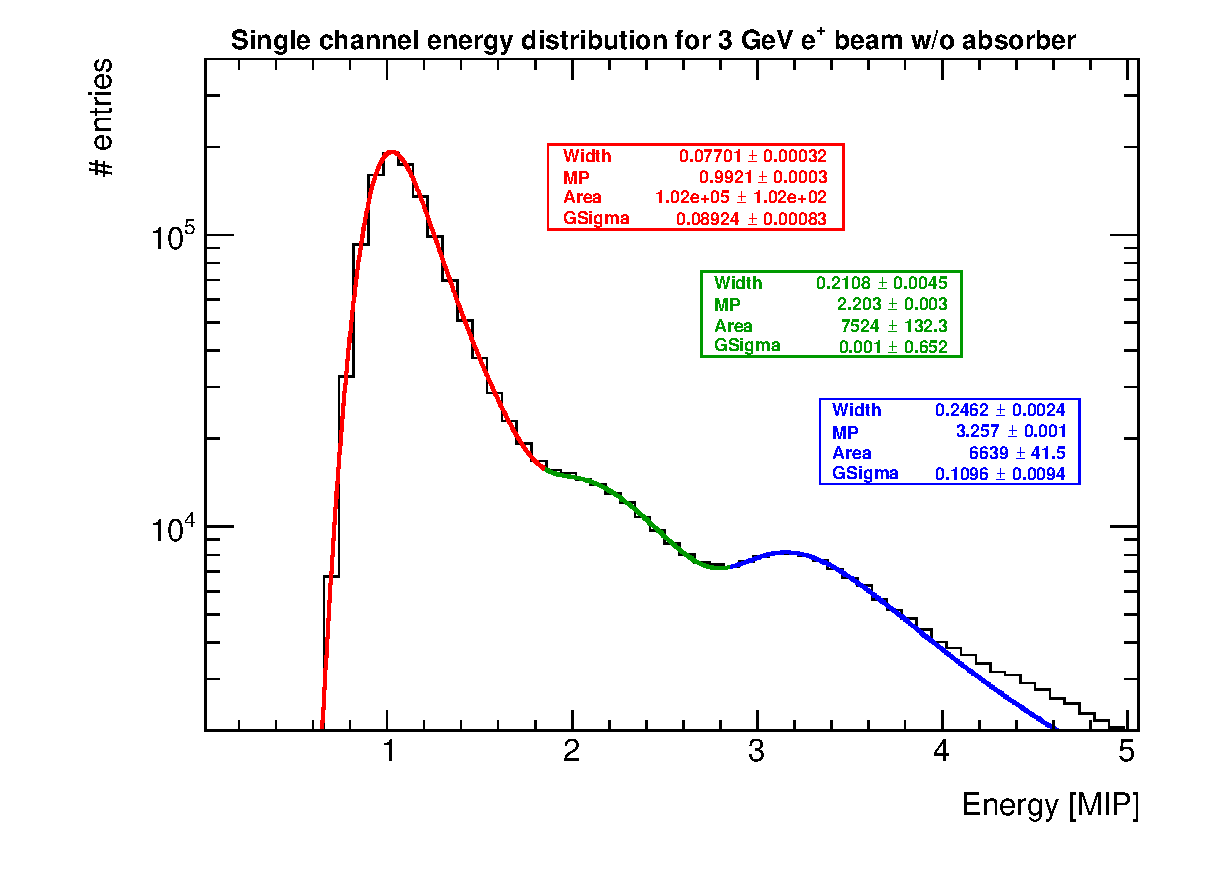
\includegraphics[width=4in]{figs/MIP/MIP3peaks.eps} 
    \end{tabular}
    \caption{The single channel energy distribution (for all calibrated channels) for 3 GeV positron tracks acting as MIPs.}
\label{mip3peaks}
\end{figure}

To evaluate 
the single hit detection efficiency we define a high purity sample of
events of positrons traversing the detector perpendicularly by selecting
tracks with at least 5 layers (of 7 possible) with a hit in exactly the same channel. Afterwards we 
check if the other layers have or not a hit in the same channel (expanding the search
to the neighbor channels) with energy larger or equal than 0.3 MIP.
Finally, we repeat this for all layers 
and channels. The results are shown in Figure \ref{efficiency}. Except few exceptions, the efficiency is 
compatible with $100\%$.
Lower efficiencies in the first layer are related to the presence of
noisy channels not well identified in the commissioning phase that boosted the filling
of the the 15 SCAs of three ASICs. In the last layer (separated from the
other layers by four slots of 1.5 cm instead of only one) we also observe few small deviations
from the $\sim100\%$ which are indeed
associated to a slight misalignment of the tracks visible only in the outliers channels. 
If we remove these channels i nthe outliers from the analysis
the full efficiency is recovered.

\begin{figure}[!t]
  \centering 
    \begin{tabular}{ll}
      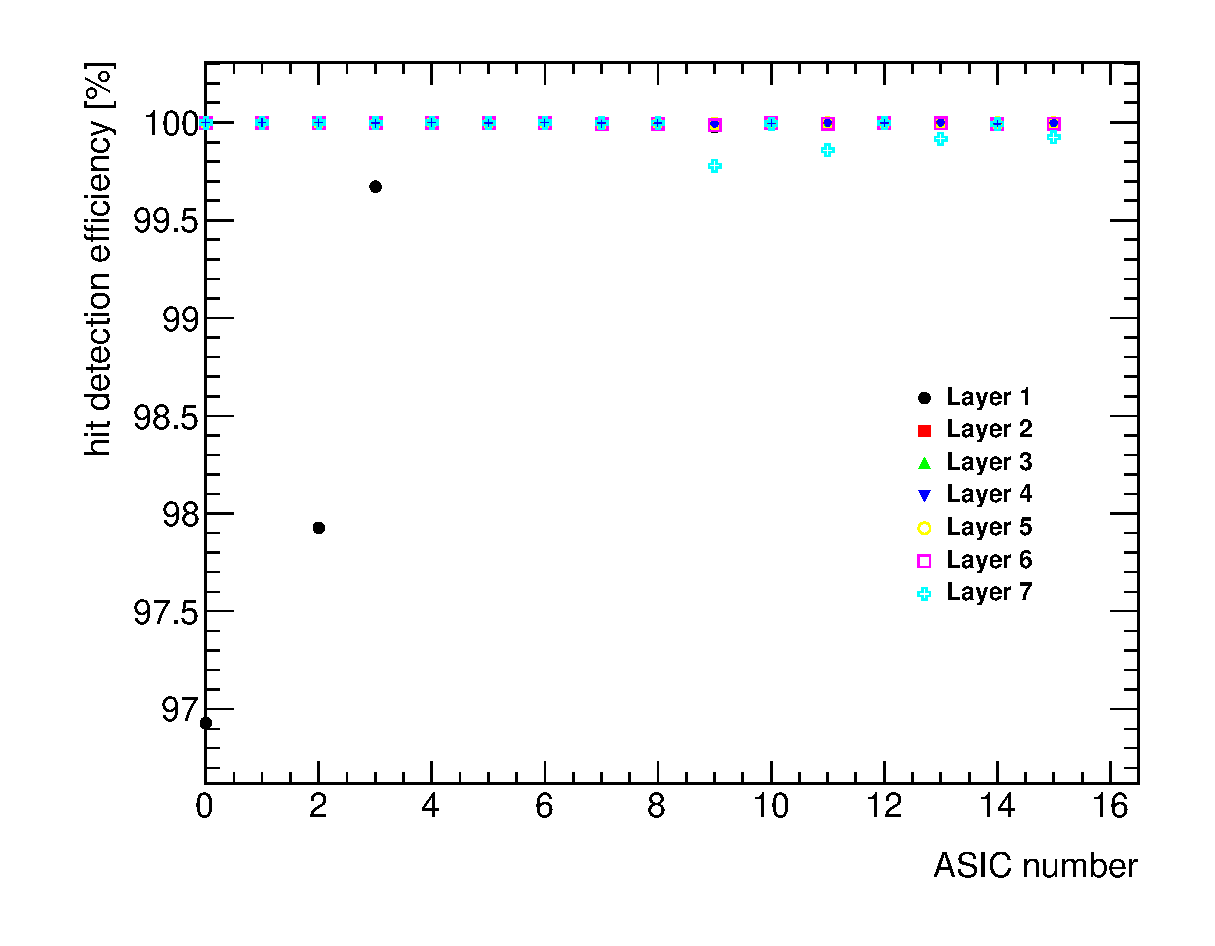
\includegraphics[width=2.8in]{figs/MIP/efficiency_nhits4_chips.eps} & 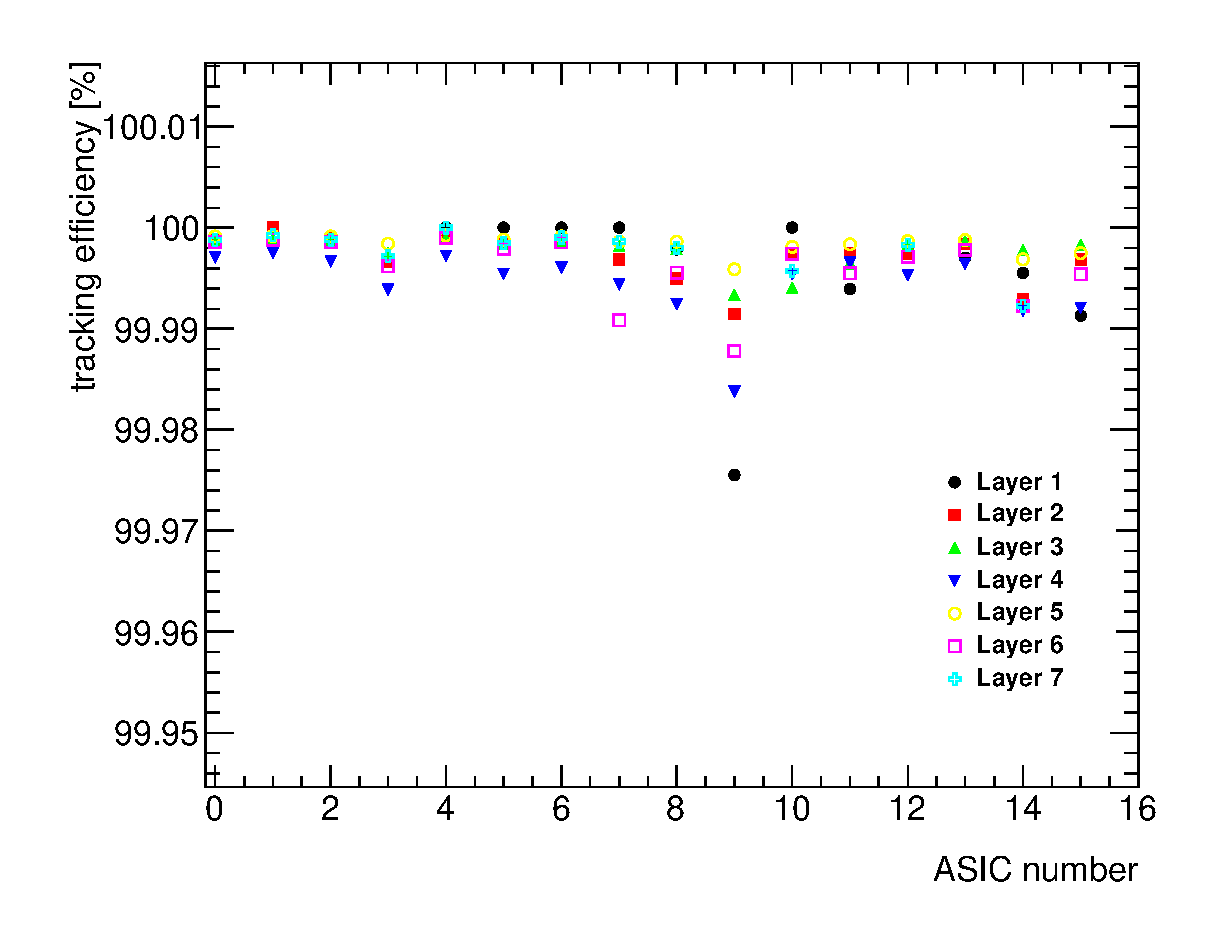
\includegraphics[width=2.8in]{figs/MIP/efficiency_nhits4_chips_zoom.eps} \\
    \end{tabular}
    \caption{Left: MIP detection efficiency for all layers and ASICs in high purity samples of tracks of MIP-like acting particles. Right: same figures with a zoom in the y-axis. In both cases, the average efficiency of the 64 channels in each ASIC is shown.}
\label{efficiency}
\end{figure}


\subsubsection{S/N ratio in the ADC}
\label{sec:mip}

The signal-over-noise ratio in the ADC (corresponding to the slow shaper of the SKIROC2) is defined 
as the ratio between the most-probable-value of
the Landau-gauss function fit to the data (pedestal subtracted) and the noise (the pedestal width). This quantity 
has been calculated for all channels and all slabs and, in average, it corresponds to 20.4.
Results are summarized in Figure \ref{mipandSN}, rightmost plot.


\subsection{Pedestal stability in electromagnetic shower events}
\label{sec:showers}

The pedestal stability in events with large amount of charge deposited by the ASICs, as are the 
electromagnetic shower events, has been also calculated. All the results shown in this section correspond to data taken during the tungsten program, 
using the W-configuration number 2 when shooting the beam in the ASIC 12 (and partially in the 13). Only the ASIC 12 is used in the analysis. For other configurations and 
positions of the beam we get comparable results. We used also a calibrated data sample were the pedestal values have been 
subtracted and the MIP calibration has been applied. 
Therefore, all energy measurements are given in MIP units and the pedestal
values are expected to be equal to zero.
In order to select a high purity of
electromagnetic shower like the events, 
we used a simple criteria: select only events with at least 6 of the layers with at least a hit with E > 0.5 MIP.

\begin{figure}[!t]
  \centering 
    \begin{tabular}{ll}
      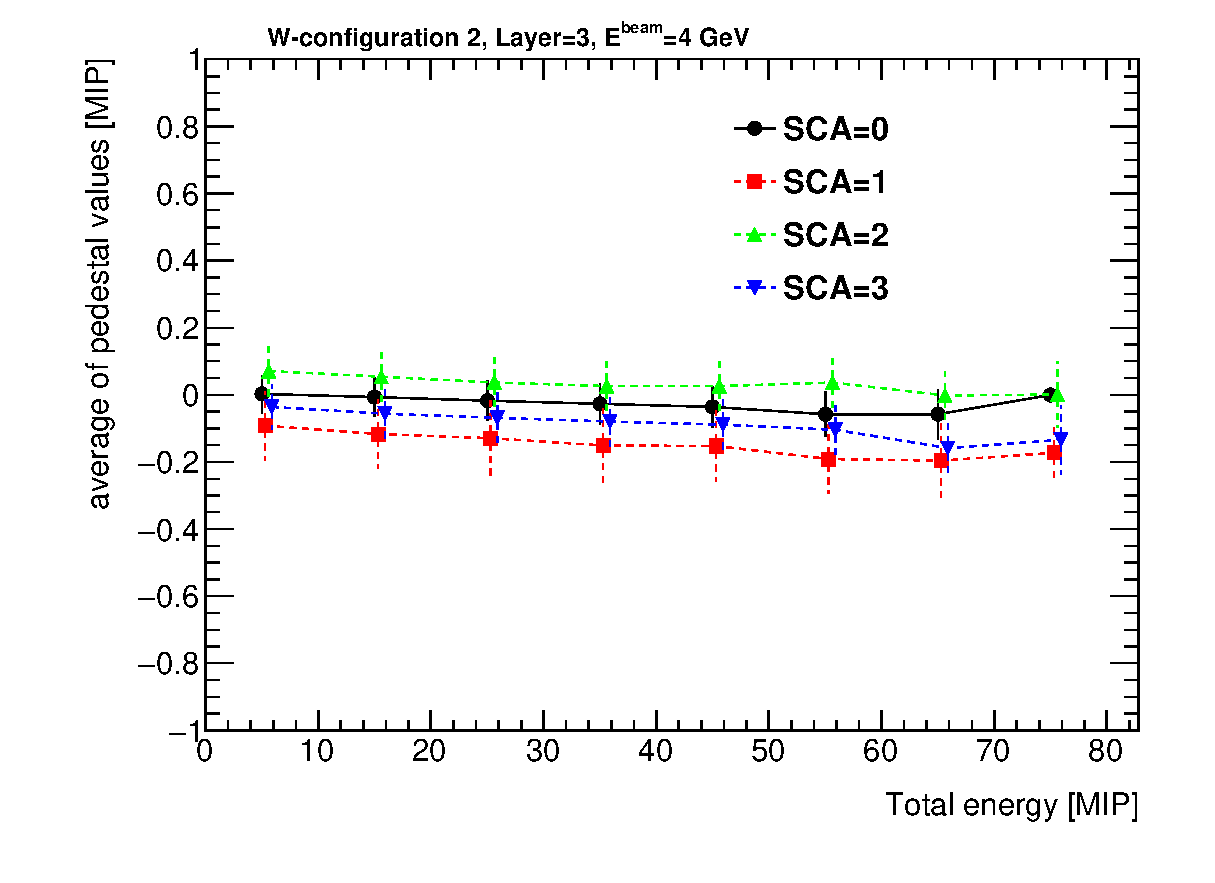
\includegraphics[width=2.8in]{figs/pedestal/pedestal_vs_energy_shower.eps} & 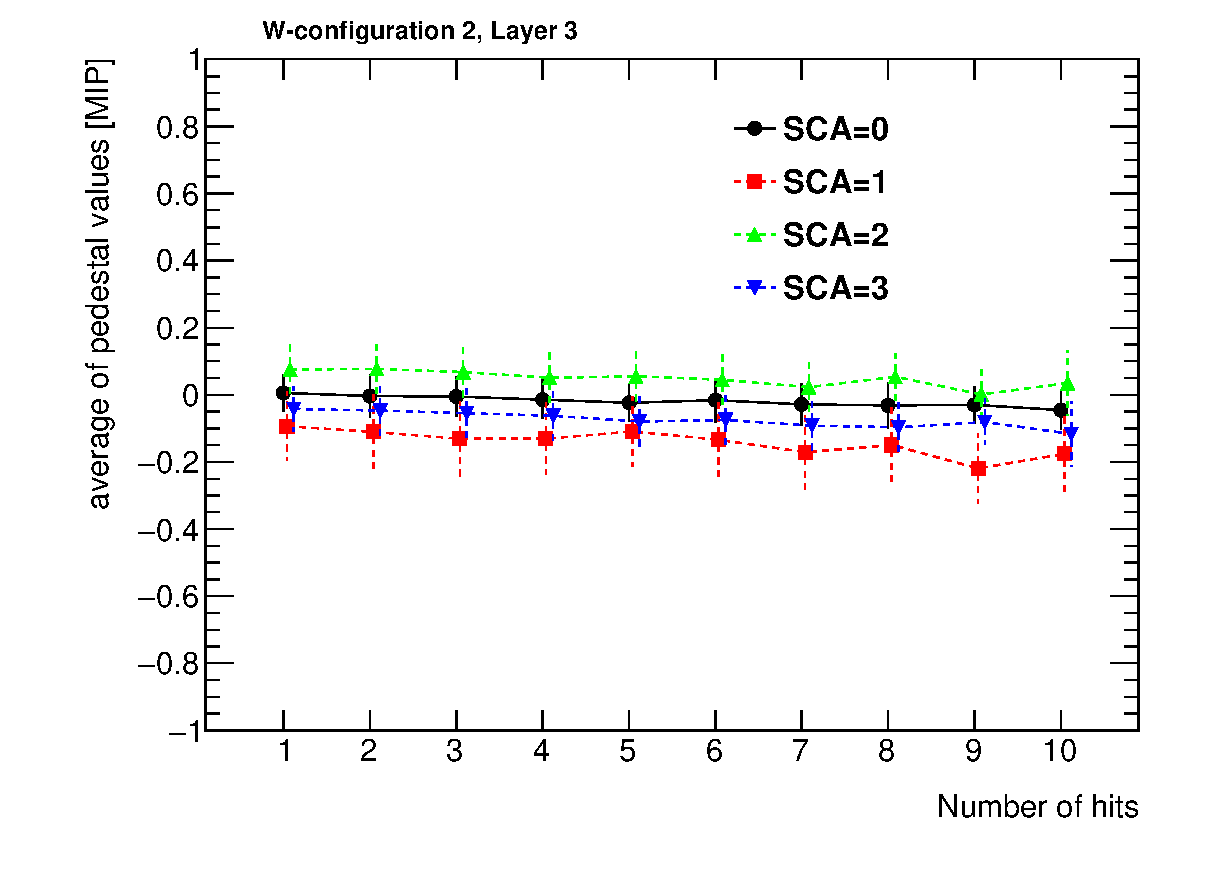
\includegraphics[width=2.8in]{figs/pedestal/pedestal_vs_nhits_shower.eps} \\
    \end{tabular}
    \caption{Left: mean position of the projection of the pedestal distribution of all channels of ASIC 12 in the Layer 3 calculated when different energies are collected in the ASIC (in bins of 10 MIPs). Right: same but as a function of the number of hits. In both cases, the results are shown for few SCA. The points for SCA larger than zero are slightly shifted in the x-axis to optimize the visualization.}
\label{pedestal_shower_1}
\end{figure}

Two main observations have been extracted from the recalculation of the pedestals and its comparison
with the values obtained previously during the calibration runs. The first observation
consists in a relatively small 
drift of the pedestal values
towards lower values when the collected energy is high (or when the number of triggered channels is large).
For events with 80 MIPs collected in the ASIC, we have an average drift of the pedestal of $\sim$ 0.05 MIP. 
This can be seen in Figure \ref{pedestal_shower_1} for several SCAs where the
average of the projection of the pedestal distribution for all channels non triggered in ASIC 12 of layer 3 
is plot as a function of the total energy measured by the ASIC (or the total number of hits).
We see that in all cases, the slopes of the curves 
for each SCA are very similar.
This is feature is known and it is due to the architecture of the SKIROC2 (and 2a) ASICs 
where high inrush of currents can slightly shift the baseline of the analogue power supply. 
This feature is foreseen to be removed from the SKIROC3 ASICs. 

The second observation extracted from this analysis can be also seen in Figure \ref{pedestal_shower_1}: in addition
to the small drift of the pedestal value an SCA-alternate global shift
is observed. This feature is still not fully understood although the fact that the effect is observed in
alternate SCAs but no time dependence has been observed hints to some issue affecting the digital part of the ASIC 
(where the SCAs enter in play). 
In Figure \ref{pedestal_shower_2} we can see the effect, SCA per SCA, for different energies of the beam
and for different layers. We see that the effect is enhanced when large amounts of charge
are deposited in the ASIC ({\it i.e.} at larger beam energies or for the layers in the maximum of the shower
profile).
Dedicated tests in the laboratory and in the beam are needed in order to clarify this issue.

\begin{figure}[!t]
  \centering 
    \begin{tabular}{ll}
      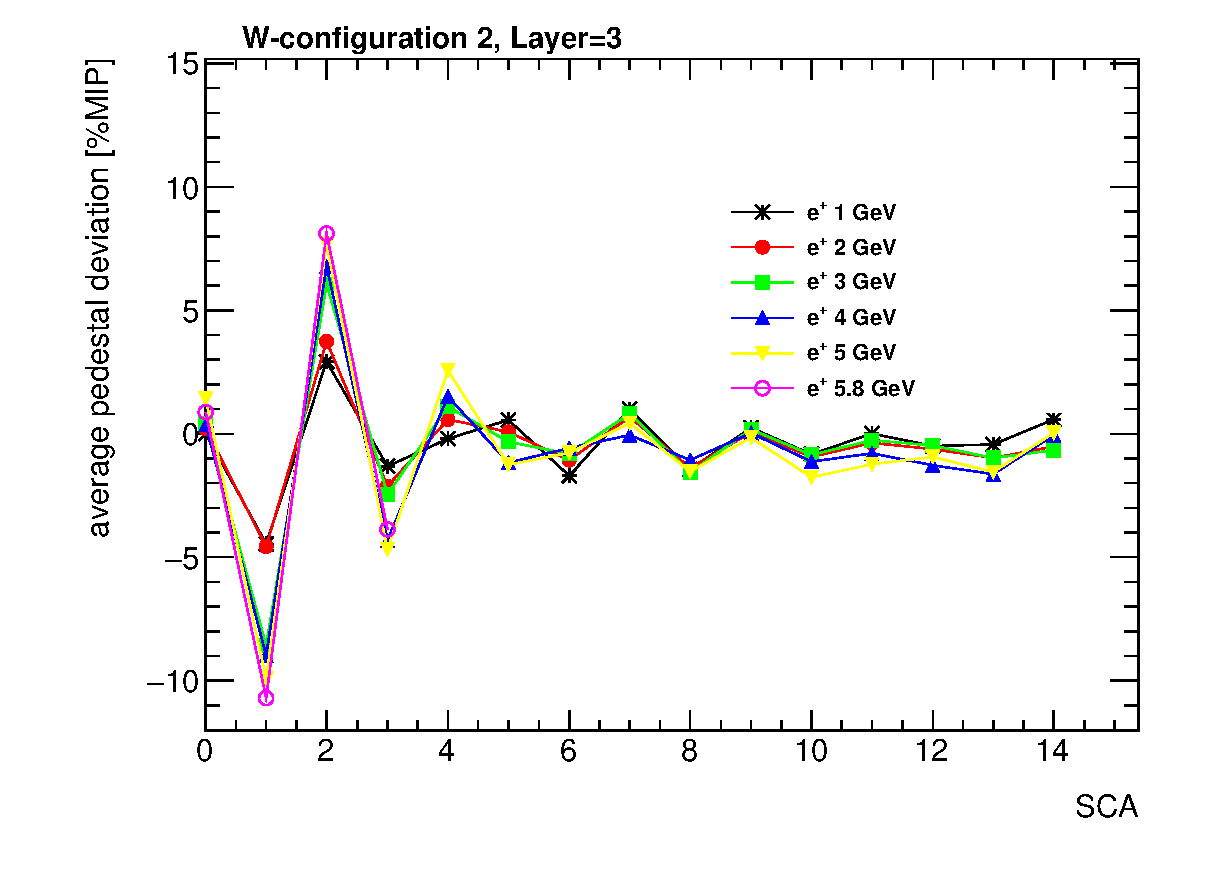
\includegraphics[width=2.8in]{figs/pedestal/pedestal_deviation_layer3.eps} & 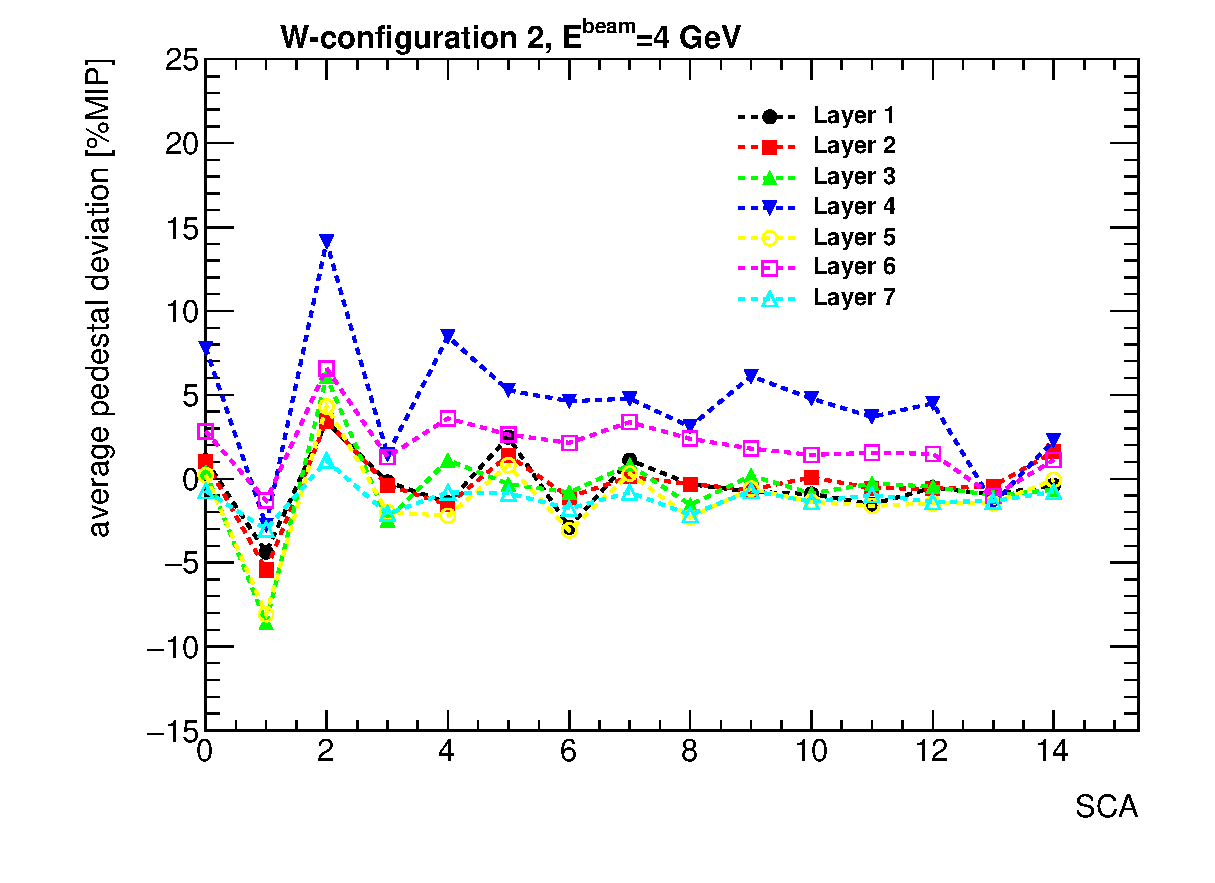
\includegraphics[width=2.8in]{figs/pedestal/pedestal_deviation_4GeV.eps} \\
    \end{tabular}
    \caption{Left: average value on each SCA of the calculated pedestals for all channels of ASIC 12 in the Layer 3 for different energies of the beam. Right: same but fixing the energy of the beam and comparing several layers.}
\label{pedestal_shower_2}
\end{figure}








\subsection{Fake triggers filtering}
\label{sec:retriggers}

Several types of fake signals have been observed in the technollogical prototype since its construction and test. A detailed description of them
can be found in previous articles, as for example, in Ref. \cite{Amjad:2014tha}. All these fake signals are easily identified
and tagged during the data acquisition and removed afterwards from the analysis
not introducing any loss of performance as can be seen, for example, in the tracking efficiency plots.
In the following, we briefly describe the status of the monitoring, debugging and filtering
of such kind of events.

\subsubsection*{Empty triggers}

Empty trigger events are a well known feature of SKIROC2. The issue appears when during
the acquisition the rising edge of the slow clock falls during the OR64 signal used
to signalize the lecture of a signal over threshold to validate the change to a new SCA.
When this happens at the end of the clock period, the change to a new SCA is validated twice.
This effect creates around 10-15\% of empty events which are easily filter and removed from the
analysis. \todo{The ratio of empty triggers in the new SKIROC2a is reduced to $\sim3\%$ by reducing
the length of the OR64 by a factor X.}

\subsubsection*{Plane events and retriggers}

Another well know issue is related to the appearance of bunches of consecutive fake triggers that
quickly fill several SCA in consecutive slow clock periods. These events are also
characterized by triggering many channels (some times even all channels of an ASIC) at the same time.
Although the ultimate reason of the appearance of these events remains unknown we have done
a lot of advances in this topic. We know that the SKIROC2 and 2a preamplifiers are referenced to the analog power supply level,
therefore, any voltage dip can ve seen as signal by the preamplifiers. The presence of a high inrush of current
due to many channels triggered at the same time can create these voltage dips.
In previous studies ({\it i.e.} reference \cite{Amjad:2014tha}), the ratio of retriggers and plane events
was reduced by improving the power supply stabilization capacitances. It is important to remark that
all layers and all ASICs analog and digital levels are powered using the same power supply.
Moreover, the high voltage power supply for the polarization of the PIN diode it is also common for all layers.
Therefore any noise in
these power supplies or any overload of an ASIC may lead participate in the creation of fake signals
in different ASICs and layers.

Studying the MIP calibration data of this beam test we have noticed that most of the retriggers and plane events are originated 
in
ASICs far from the beam spot. Even more, hot spots tend appear near the channels 37 and the channels tagged as ``underflowed'' 
during
the commissioning phase. The amount these events have been estimated to be of $1-3\%$ in the ASICs where high frequency
interactions are produced ({\it i.e.} using 3 GeV positrons ate 2-3 KHz) and at higher rates even larger than $40\%$ in other 
ASICs far from the beam spot.
Moreover, it has been noticed a correlation between the time that an ASIC was full and the time of the appearance of some 
retriggers in other areas of the PCB. 
This correlation corresponds to $\sim8$ BCIDs (1.6 $\mu$s) which hints
of a distortion on the analogue power supply when
the signal that informs the DIF that one ASIC memory has been filled is transmitted from the ASICs to
the DIF through the PCB.


All this information and dedicated studies in the laboratory will be used for the
improvement of the power delivery, the PCB design and for further SKIROC developments 
with the possible approval the ILC in the scope.


\section{Summary and prospects}
\label{sec:prospects}

The R\&D program of the highly granular SiW-ECAL detector is in an exciting phase. 
After the proof of principle of the imaging calorimetry concept using the physics prototype, the 
technological prototype is being constructed and tested. In this document we describe the commissioning and
beam test performance of a prototype built in with the first fully assembled
detector elements (still only 7 over the total of $\sim$10000 to be in the ILD).

A very comprehensive and detailed commissioning procedure has been established and optimized
allowing us to identify and isolate the different noise sources that could spoil the data taking.
The beam test has provided a lot of useful data, allowing first for the study of 
the performance of the detector and secondly 
for its channel by channel calibration. 
A full analysis including the comparison with simulations of the 
second part of the data taking program (the electromagnetic showers) is to come.
During both phases, the commissioning and the beam test,
we have collected a good amount of data and results
that will serve as input for future improvements on
the design of the ASUs, the SKIROC and the upstream DAQ.

In parallel to the work described here, several R\&D efforts are being carried.
For example, we know that the ILD ECAL will host long layers of up to $\sim$2.5m.
A long layer constitutes a technological challenge in both aspects, the mechanical
(very thin and long structure with fragile sensors in the bottom, complicated assembly procedure...)
and the electrical (i.e. transmission of signals and high currents).
For example, interconnections between ASUs and between ASU and interface card are one of
the most involved parts of the assembly
and require close collaboration between mechanical and electronic engineers.
Therefore, many efforts are focused in the construction and test of such long 
layers made of chains of ASUs (up to $\sim$15 ASU) 
as well as in the standardization of the interconnections. 
In addition, many efforts in the compactification of
the DAQ and the ASUs ({\it i.e.} the chip on board versions of the 
ASUs described in Section \ref{sec:ASU}) are being
conducted by the SiW-ECAL collaboration.


\acknowledgments

This project has received funding from the European Union{\textquotesingle}s Horizon 2020 Research and Innovation program under Grant Agreement no. 654168.
This work was supported by the P2IO LabEx (ANR-10-LABX-0038), excellence project HIGHTEC,
in the framework {\textquotesingle}Investissements d{\textquotesingle}Avenir{\textquotesingle}
(ANR-11-IDEX-0003-01) managed by the French National Research Agency (ANR).
The research leading to these results has received funding from the People Programme (Marie
Curie Actions) of the European Union{\textquotesingle}s Seventh Framework Programme (FP7/2007-2013)
under REA grant agreement, PCOFUND-GA-2013-609102, through the PRESTIGE
programme coordinated by Campus France.
The measurements leading to these results have been performed at the Test Beam Facility at DESY Hamburg (Germany), a member of the Helmholtz Association (HGF).


% We suggest to always provide author, title and journal data:
% in short all the informations that clearly identify a document.

\bibliographystyle{JHEP}
\bibliography{references}

\end{document}
